\noindent Viele Aufgaben des Design For Six Sigma sind mehrdimensional. Deshalb wird das Vorgehen der eindimensionalen Aufgabenstellungen auf mehrdimensionale Regressionsmodelle erweitert. Dabei wird auch gezeigt, wie Polynome als Regressionsfunktion eingesetzt und bewertet werden k\"{o}nnen.

\subsection{Bestimmung der Regressionsfunktion}

\noindent Die Herleitung der Regressionsfunktion f\"{u}r mehrdimensionale Datens\"{a}tze wird genauso durchgef\"{u}hrt wie bei eindimensionalen Datens\"{a}tzen. Aufgrund der unterschiedlichen Eingangsvariablen ist die Bezeichnung der Variablen komplizierter. Um eine effiziente Darstellungsform zu erhalten, wird deshalb die Matrizenrechnung eingesetzt. Die erforderlichen Grundlagen der linearen Algebra sind im Anhang zusammengefasst.

\subsubsection{Modellansatz und Datenstruktur}

\noindent Ausgangspunkt f\"{u}r mehrdimensionale Regressionsfunktionen ist ein Prozess, dessen Ausgangssignal y durch M Eingangsgr\"{o}{\ss}en $x_{m}$ und einem Messfehler e beschreiben wird.

\begin{equation}\label{eq:thirteenone}
y=\beta _{0} +\beta _{1} \cdot x_{1} +\ldots +\beta _{m} \cdot x_{m} +\ldots +\beta _{M} \cdot x_{M} +e
\end{equation}

\noindent Dabei ist e ein zuf\"{a}lliger Fehler, der einen Mittelwert $\mu_{e} = 0$ und eine unbekannte konstante Varianz $\sigma^{2}$ aufweist. Die Regressionskoeffizienten $\beta_{m}$ werden auf Basis einer Stichprobe gesch\"{a}tzt. Da M + 1 Regressionsparameter gesch\"{a}tzt werden m\"{u}ssen, sind mindestens N = M + 1 Stichproben erforderlich. Jede Stichprobe besteht aus einem Satz von Eingangsgr\"{o}{\ss}en $x_{n1} \dots x_{nM}$ und einem Messwert der Zielgr\"{o}{\ss}e $y_{n}$. Die Eingangswerte werden in der Matrix X

\begin{equation}\label{eq:thirteentwo}
\mathbf{X}=
\begin{pmatrix}
1 & \cdots & x_{1m} & \cdots & x_{1M} \\
\vdots & \ddots & \vdots & & \vdots \\
1 & \cdots & x_{nm} & \cdots & x_{nM}\\
\vdots & & \vdots & \ddots & \vdots\\
1 & \cdots & x_{Nm} & \cdots & x_{NM}\\
\end{pmatrix}
\end{equation}

\noindent und die Zielgr\"{o}{\ss}en in einem Vektor \underbar{y}

\begin{equation}\label{eq:thirteenthree}
\underline{y}=
\begin{pmatrix}
y_{1}\\
\vdots\\
y_{n}\\
\vdots\\
y_{N}\\
\end{pmatrix}
\end{equation}

\noindent zusammengefasst. Ziel der Regressionrechnung ist es, Sch\"{a}tzwerte $b_{m}$ f\"{u}r die Regressionsparameter $\beta_{m}$ zu finden. 

\begin{equation}\label{eq:thirteenfour}
y\left(\underline{x}^{T} \right)=b_{0} +b_{1} \cdot x_{1} +\ldots +b_{m} \cdot x_{m} +\ldots +b_{M} \cdot x_{M}
\end{equation}

\noindent Dazu wird folgendes Gleichungssystem aufgebaut:

\begin{equation}\label{eq:thirteenfive}
\begin{split}
\underline{y} & = \left(\begin{array}{c} {y_{1} } \\ {\vdots } \\ {y_{n} } \\ {\vdots } \\ {y_{N} } \end{array}\right)=\left(\begin{array}{c} {b_{0} +b_{1} \cdot x_{11} +\ldots +b_{m} \cdot x_{1m} +\ldots +b_{M} \cdot x_{1M} +r_{1} } \\ {\vdots } \\ {b_{0} +b_{1} \cdot x_{n1} +\ldots +b_{m} \cdot x_{nm} +\ldots +b_{M} \cdot x_{nM} +r_{n} } \\ {\vdots } \\ {b_{0} +b_{1} \cdot x_{N1} +\ldots +b_{m} \cdot x_{Nm} +\ldots +b_{M} \cdot x_{NM} +r_{N} } \end{array}\right) \\ 
& = \left(\begin{array}{ccccc} {1} & {\cdots } & {x_{1m} } & {\cdots } & {x_{1M} } \\ {\vdots } & {\ddots } & {\vdots } & {} & {\vdots } \\ {1} & {\cdots } & {x_{nm} } & {\cdots } & {x_{nM} } \\ {\vdots } & {} & {\vdots } & {\ddots } & {\vdots } \\ {1} & {\cdots } & {x_{Nm} } & {\cdots } & {x_{NM} } \end{array}\right)\cdot \left(\begin{array}{c} {b_{0} } \\ {\vdots } \\ {b_{m} } \\ {\vdots } \\ {b_{M} } \end{array}\right)+\left(\begin{array}{c} {r_{1} } \\ {\vdots } \\ {r_{n} } \\ {\vdots } \\ {r_{N} } \end{array}\right)=\mathbf{X} \cdot \underline{b}+\underline{r}    
\end{split}
\end{equation}

\noindent Die Regressionsfunktion mit den Sch\"{a}tzwerten $b_{m}$ kann die Stichprobenwerte nicht perfekt abbilden kann. Wie im eindimensionalen Fall werden die Abweichungen als Residuen $r_{n}$ bezeichnet.

\subsubsection{Herleitung der Bestimmungsgleichung}

\noindent Zur Bestimmung der Regressionsgleichung wird die Quadratsumme der Residuen minimiert. Die Residuen errechnen sich aus der Differenz des gemessenen Wertes $y_{n}$ und dem Wert der Regeressionsfunktion an der entsprechenden Stelle

\begin{equation}\label{eq:thirteensix}
\underline{r}=\underline{y}-\mathbf{X}\cdot \underline{b}
\end{equation}

\noindent Die Quadratsumme kann als Innenprodukt dargestellt werden.

\begin{equation}\label{eq:thirteenseven}
\begin{split}
a & =\underline{r}^{T} \cdot \underline{r}=\left(\underline{y}-\mathbf{X}\cdot \underline{b}\right)^{T} \cdot \left(\underline{y}-\mathbf{X}\cdot \underline{b}\right)=\left(\underline{y}^{T} -\underline{b}^{T} \cdot \mathbf{X}^{T} \right)\cdot \left(\underline{y}-\mathbf{X}\cdot \underline{b}\right) \\ 
& = \underline{y}^{T} \cdot \underline{y}-\underline{y}^{T} \cdot \mathbf{X}\cdot \underline{b}-\underline{b}^{T} \cdot \mathbf{X}^{T} \cdot \underline{y}+\underline{b}^{T} \cdot \mathbf{X}^{T} \cdot \mathbf{X}\cdot \underline{b}    
\end{split}
\end{equation}

\noindent Wegen der Beziehung

\begin{equation}\label{eq:thirteeneight}
\underline{y}^{T} \cdot \mathbf{X}\cdot \underline{b}=\underline{b}^{T} \cdot \mathbf{X}^{T} \cdot \underline{y}
\end{equation}

\noindent ergibt sich f\"{u}r die Quadratsumme der Residuen

\begin{equation}\label{eq:thirteennine}
\begin{split}
a & = \underline{r}^{T} \cdot \underline{r}=\left(\underline{y}-\mathbf{X}\cdot \underline{b}\right)^{T} \cdot \left(\underline{y}-\mathbf{X}\cdot \underline{b}\right)=\left(\underline{y}^{T} -\underline{b}^{T} \cdot \mathbf{X}^{T} \right)\cdot \left(\underline{y}-\mathbf{X}\cdot \underline{b}\right) \\ 
& = \underline{y}^{T} \cdot \uy-2\cdot \ub^{T} \cdot \mathbf{X}^{T} \cdot \uy+\ub^{T} \cdot \mathbf{X}^{T} \cdot \mathbf{X}\cdot \ub
\end{split}
\end{equation}

\noindent Die Regressionsparameter $b_{m}$ werden so gew\"{a}hlt, dass die Summe a der quadratischen Fehler minimal wird. Notwendige Bedingung f\"{u}r ein Minimum ist, dass die partielle Ableitungen von a nach $b_{m}$ null werden. Es entstehen M + 1 Gleichungen f\"{u}r M + 1 unbekannte Parameter $b_{m}$. Aus diesem Ansatz folgt die Gleichung 

\begin{equation}\label{eq:thirteenten}
\frac{\partial a}{\partial \ub} =-2\cdot \mathbf{X}^{T} \cdot \uy+2\cdot \mathbf{X}^{T} \cdot \mathbf{X}\cdot \ub=0
\end{equation}

\noindent beziehungsweise

\begin{equation}\label{eq:thirteeneleven}
\mathbf{X}^{T} \cdot \mathbf{X}\cdot \ub=\mathbf{X}^{T} \cdot \uy
\end{equation}

\noindent F\"{u}r den Fall, dass die Inverse von $\mathbf{X}^{T}\cdot \mathbf{X}$ existiert, ergibt sich die Bestimmungsgleichung 

\begin{equation}\label{eq:thirteentwelve}
\ub=\left(\mathbf{X}^{T} \cdot \mathbf{X}\right)^{-1} \cdot \mathbf{X}^{T} \cdot \uy
\end{equation}

\noindent Dabei sind die Parameter $b_{m}$ Sch\"{a}tzwerte f\"{u}r die Parameter $\beta_{m}$ des zugrundeliegenden Prozesses.\bigskip

\noindent
\colorbox{lightgray}{%
\arrayrulecolor{white}%
\renewcommand\arraystretch{0.6}%
\begin{tabular}{ wl{16.5cm} }
{\fontfamily{phv}\selectfont
\noindent{Beispiel: Invertierender Verst\"{a}rker}}
\end{tabular}%
}\medskip

\noindent Als Beispiel wird ein invertierender Verst\"{a}rker aufgegriffen. Es wird die Abh\"{a}ngigkeit der Ausgangsspannung $U_{A}$ von der Eingangsspannung $U_{E}$ und der Offsetspannung $U_{OFF}$ beschrieben.

\begin{equation}\label{eq:thirteenthirteen}
U_{A} =-\frac{R_{2}}{R_{1}} \cdot U_{E} +\left(1+\frac{R_{2}}{R_{1}} \right)\cdot U_{OFF}
\end{equation}

\noindent Die Funktion soll \"{u}ber eine Regressionsrechnung ermittelt werden. Dazu wird eine Schaltung mit den Widerst\"{a}nden $R_{1} = 10 k\Omega$ und $R_{2} = 1 k\Omega$ aufgebaut. Es ergeben sich die in Tabelle \ref{tab:thirteenone} dargestellten Messwerte.

\begin{table}[H]
\setlength{\arrayrulewidth}{.1em}
\caption{Ausgangsspannung eines invertierenden Operationsverst\"{a}rkers als Beispiel f\"{u}r eine zweidimensionale lineare Regression}
\setlength{\fboxsep}{0pt}%
\colorbox{lightgray}{%
\arrayrulecolor{white}%
\begin{tabular}{ wc{3.9cm} | wc{3.9cm} | wc{3.9cm} | wc{3.9cm} }
\hline\xrowht{10pt}

\fontfamily{phv}\selectfont\textbf{Index} &
\fontfamily{phv}\selectfont\textbf{U$_{\textbf{A}}$ / mV} &
\fontfamily{phv}\selectfont\textbf{U$_{\textbf{OFF}}$ / mV} &
\fontfamily{phv}\selectfont\textbf{U$_{\textbf{E}}$ / mV} \\ \hline \xrowht{10pt}

\fontfamily{phv}\selectfont{1} & \fontfamily{phv}\selectfont{5.5954} & \fontfamily{phv}\selectfont{0} & \fontfamily{phv}\selectfont{- 50}\\ \hline\xrowht{10pt}

\fontfamily{phv}\selectfont{2} & \fontfamily{phv}\selectfont{- 5.6012} & \fontfamily{phv}\selectfont{0} & \fontfamily{phv}\selectfont{50}\\ \hline\xrowht{10pt}

\fontfamily{phv}\selectfont{3} & \fontfamily{phv}\selectfont{4.9901} & \fontfamily{phv}\selectfont{0} & \fontfamily{phv}\selectfont{- 50}\\ \hline\xrowht{10pt}

\fontfamily{phv}\selectfont{4} & \fontfamily{phv}\selectfont{- 5.0784} & \fontfamily{phv}\selectfont{0} & \fontfamily{phv}\selectfont{50}\\ \hline\xrowht{10pt}

\fontfamily{phv}\selectfont{5} & \fontfamily{phv}\selectfont{15.1980} & \fontfamily{phv}\selectfont{10} & \fontfamily{phv}\selectfont{- 50}\\ \hline\xrowht{10pt}

\fontfamily{phv}\selectfont{6} & \fontfamily{phv}\selectfont{6.1287} & \fontfamily{phv}\selectfont{10} & \fontfamily{phv}\selectfont{50}\\ \hline\xrowht{10pt}

\fontfamily{phv}\selectfont{7} & \fontfamily{phv}\selectfont{15.4718} & \fontfamily{phv}\selectfont{10} & \fontfamily{phv}\selectfont{-50}\\ \hline\xrowht{10pt}

\fontfamily{phv}\selectfont{8} & \fontfamily{phv}\selectfont{6.7076} & \fontfamily{phv}\selectfont{10} & \fontfamily{phv}\selectfont{50}\\ \hline\xrowht{10pt}

\fontfamily{phv}\selectfont{9} & \fontfamily{phv}\selectfont{5.0975} & \fontfamily{phv}\selectfont{5} & \fontfamily{phv}\selectfont{0}\\ \hline

\end{tabular}%
}
\label{tab:thirteenone}
\end{table}

\noindent Unter Ber\"{u}cksichtigung der Konstante $b_{0}$ ergibt sich die Matrix \textbf{X} 

\begin{equation}\label{eq:thirteenfourteen}
X=\left(\begin{array}{ccc} {1} & {0} & {-50} \\ {1} & {0} & {50} \\ {1} & {0} & {-50} \\ {1} & {0} & {50} \\ {1} & {10} & {-50} \\ {1} & {10} & {50} \\ {1} & {10} & {-50} \\ {1} & {10} & {50} \\ {1} & {5} & {0} \end{array}\right)
\end{equation}

\noindent und der Vektor \underbar{y} zu

\begin{equation}\label{eq:thirteenfifteen}
\underline{y}=\left(\begin{array}{c} {5.5954} \\ {-5.6012} \\ {4.9901} \\ {-5.0784} \\ {15.1980} \\ {6.12875} \\ {15.4718} \\ {6.7076} \\ {5.0975} \end{array}\right)
\end{equation}

\noindent Der Vektor \underbar{b} der unbekannten Parameter berechnet sich zu

\begin{equation}\label{eq:thirteensixteen}
\underline{b}=\left(X^{T} \cdot X\right)^{-1} \cdot X^{T} \cdot \underline{y}=\left(\begin{array}{c} {-0.0601} \\ {1.0900} \\ {-0.0977} \end{array}\right)
\end{equation}

\noindent Die Regressionsfl\"{a}che der gesch\"{a}tzten Ausgangsspannung $U_{A}$ ergibt sich aus 

\begin{equation}\label{eq:thirteenseventeen}
U_{A} \left(U_{E} ,U_{OFF} \right)=X\cdot \underline{b}=-0.0601+1.0900\cdot U_{OFF} -0.0977\cdot U_{E}
\end{equation}

\noindent Die \"{u}ber die Regressionsfunktion berechnete Ausgangsspannung und die \"{u}ber Gleichung \eqref{eq:thirteenthirteen} berechnete Ausgangsspannung sind in Bild \ref{fig:Verstaerkerschaltung} zum Vergleich dargestellt.

\clearpage

\noindent 
\begin{figure}[H]
  \centerline{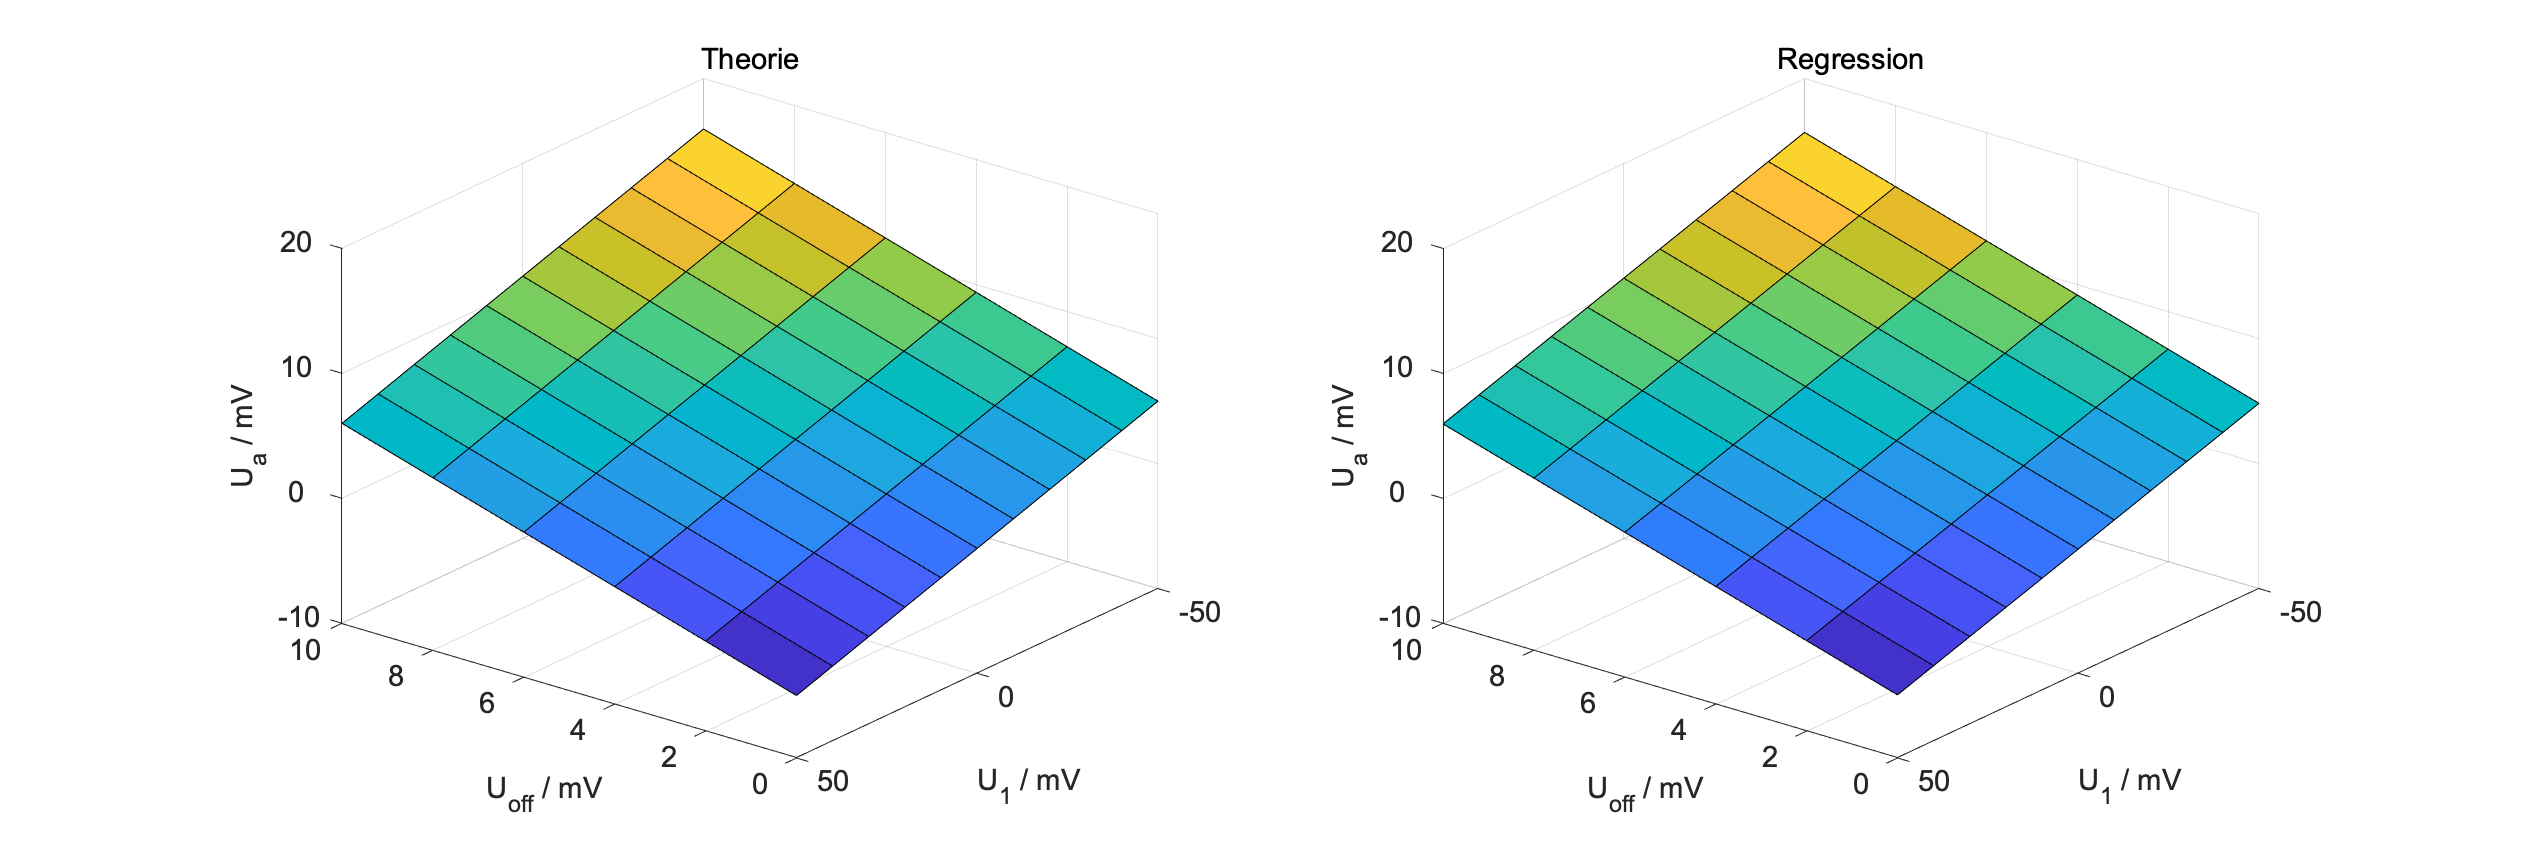
\includegraphics[width=1\textwidth]{Kapitel13/Bilder/image1}}
  \caption{Ausgangsspannung eines invertierenden Verst\"{a}rkers\\
  a) Theoretische Rechnung\\
  b) Regressionsrechnung auf Basis der Messwerte in Tabelle \ref{tab:thirteenone}}
  \label{fig:Verstaerkerschaltung}
\end{figure}

\noindent Aufgrund der Messfehler, die bei der Bestimmung der Ausgangsspannung in Tabelle \ref{tab:thirteenone} gemacht wurden, stimmt die Regressionsgleichung nicht exakt mit der idealen Gleichung

\begin{equation}\label{eq:thirteeneighteen}
U_{A} =\left(1+\frac{R_{2}}{R_{1}} \right)\cdot U_{OFF} -\frac{R_{2} }{R_{1}} \cdot U_{E} =1.1\cdot U_{OFF} -0.1\cdot U_{E}
\end{equation}

\noindent \"{u}berein. Die bestimmte Regressionsfunktion stellt aber eine gute N\"{a}herung der analytischen Gleichung dar. 

\subsubsection{Geometrische Interpretation der Bestimmungsgleichung}

\noindent $<<<$ Orthogonale Projektion $>>>$

\subsubsection{Mathematischer Ansatz f\"{u}r mehrdimensionale Regressionsfunktionen}

\noindent Zur besseren \"{U}bersicht wird im vorangegangenen Abschnitt eine zweidimensionale, lineare Funktion verwendet, um eine Regressionsfl\"{a}che zu berechnen. In der Praxis werden aber Funktionen verwendet, die neben der linearen Abh\"{a}ngigkeit von Eingangsgr\"{o}{\ss}en auch quadratische Abh\"{a}ngigkeiten und Wechselwirkungen abbilden. Die Beschreibung der Zielgr\"{o}{\ss}e erfolgt damit f\"{u}r Systeme mit zwei Eingangsgr\"{o}{\ss}en \"{u}ber eine Gleichung der Form

\begin{equation}\label{eq:thirteennineteen}
y\left(\underline{x}^{T} \right)=b_{0} +b_{1} \cdot x_{1} +b_{2} \cdot x_{2} +b_{3} \cdot x_{1} \cdot x_{2} +b_{4} \cdot x_{1}^{2} +b_{5} \cdot x_{2}^{2}
\end{equation}

\noindent Dieser quadratische Funktionsansatz geht auf die Taylorreihe zur\"{u}ck. Sie wird verwendet, um Funktionen in der Umgebung definierter Punkte durch Potenzreihen darzustellen. Bei der Taylorreihe handelt es sich um eine lokal g\"{u}ltige Approximation der Funktion. Trotzdem ist die Taylorreihe ein oftmals ausreichender Ansatz, weil die Zielgr\"{o}{\ss}e y nur in einem definierten Bereich beschrieben werden soll. Die Funktion kann dabei von mehreren unabh\"{a}ngigen Eingangsgr\"{o}{\ss}en $x_{m}$ abh\"{a}ngen. Der Funktionsansatz wie in Gleichung \eqref{eq:thirteennineteen} ist damit mathematisch zul\"{a}ssig und in vielen F\"{a}lle wegen der unbekannten Abh\"{a}ngigkeit die einzige M\"{o}glichkeit, die Zielgr\"{o}{\ss}e y zu beschreiben.\newline

\noindent Der Modellansatz in Gleichung \eqref{eq:thirteennineteen} hat dar\"{u}ber hinaus den Vorteil, dass das Modell mathematisch einfach handhabbar ist. Das erleichtert zum einen f\"{u}r die Bestimmung der Modellfunktion. Zum anderen hat diese einfache mathematische Beschreibung den Vorteil, dass sie auf wenig komplexen mathematischen Operationen aufbaut. Sie kann damit auch in einfachen Systemen wie etwa der Motorsteuerung oder in Steuerungen von Haushaltsger\"{a}ten eingesetzt werden.\newline

\noindent Der Funktionsansatz in Gleichung \eqref{eq:thirteennineteen} besteht aus Termen, die bis zur zweiten Ordnung gehen. Er wird deshalb als vollquadratischer Funktionsansatz bezeichnet. Um den funktionalen Zusammenhang optimieren zu k\"{o}nnen, muss der Anwender eine Vorstellung von der mathematischen Gestalt unterschiedlicher Funktionsans\"{a}tze haben. Deshalb werden einige Funktionsans\"{a}tze kurz vorgestellt. Dabei beschr\"{a}nken sich die Darstellungen auf zwei Eingangsgr\"{o}{\ss}en und eine Zielgr\"{o}{\ss}e, um eine r\"{a}umliche Darstellung zu erm\"{o}glichen. Die hier f\"{u}r zwei Eingangsgr\"{o}{\ss}en dargestellten Ans\"{a}tze lassen sich aber auf beliebig viele Eingangsgr\"{o}{\ss}en erweitern.\bigskip

{\fontfamily{phv}\selectfont
\noindent\textbf{Linearer Modellansatz}} \smallskip

\noindent Ein linearer Ansatz zeichnet sich dadurch aus, dass die Zielgr\"{o}{\ss}e \"{u}ber lineare Terme beschrieben werden kann. Die beiden Eingangsgr\"{o}{\ss}en haben keine Wechselwirkung. Mathematisch wird dieser Ansatz beschrieben \"{u}ber

\begin{equation}\label{eq:thirteentwenty}
y=b_{0} +b_{1} \cdot x_{1} +b_{2} \cdot x_{2}
\end{equation}

\noindent Bild \ref{fig:Funktionsansatz} stellt die lineare Funktion 

\begin{equation}\label{eq:thirteentwentyone}
y=2.5+x_{1} +x_{2}
\end{equation}

\noindent grafisch dar. Entlang der Achsen entsprechen die Koeffizienten $b_{1}$ und $b_{2}$ den Koeffizienten der Steigung der Fl\"{a}che. Die Zielgr\"{o}{\ss}e steigt unabh\"{a}ngig von der Variable $x_{2}$ linear mit der Variable $x_{1}$ an.

\noindent 
\begin{figure}[H]
  \centerline{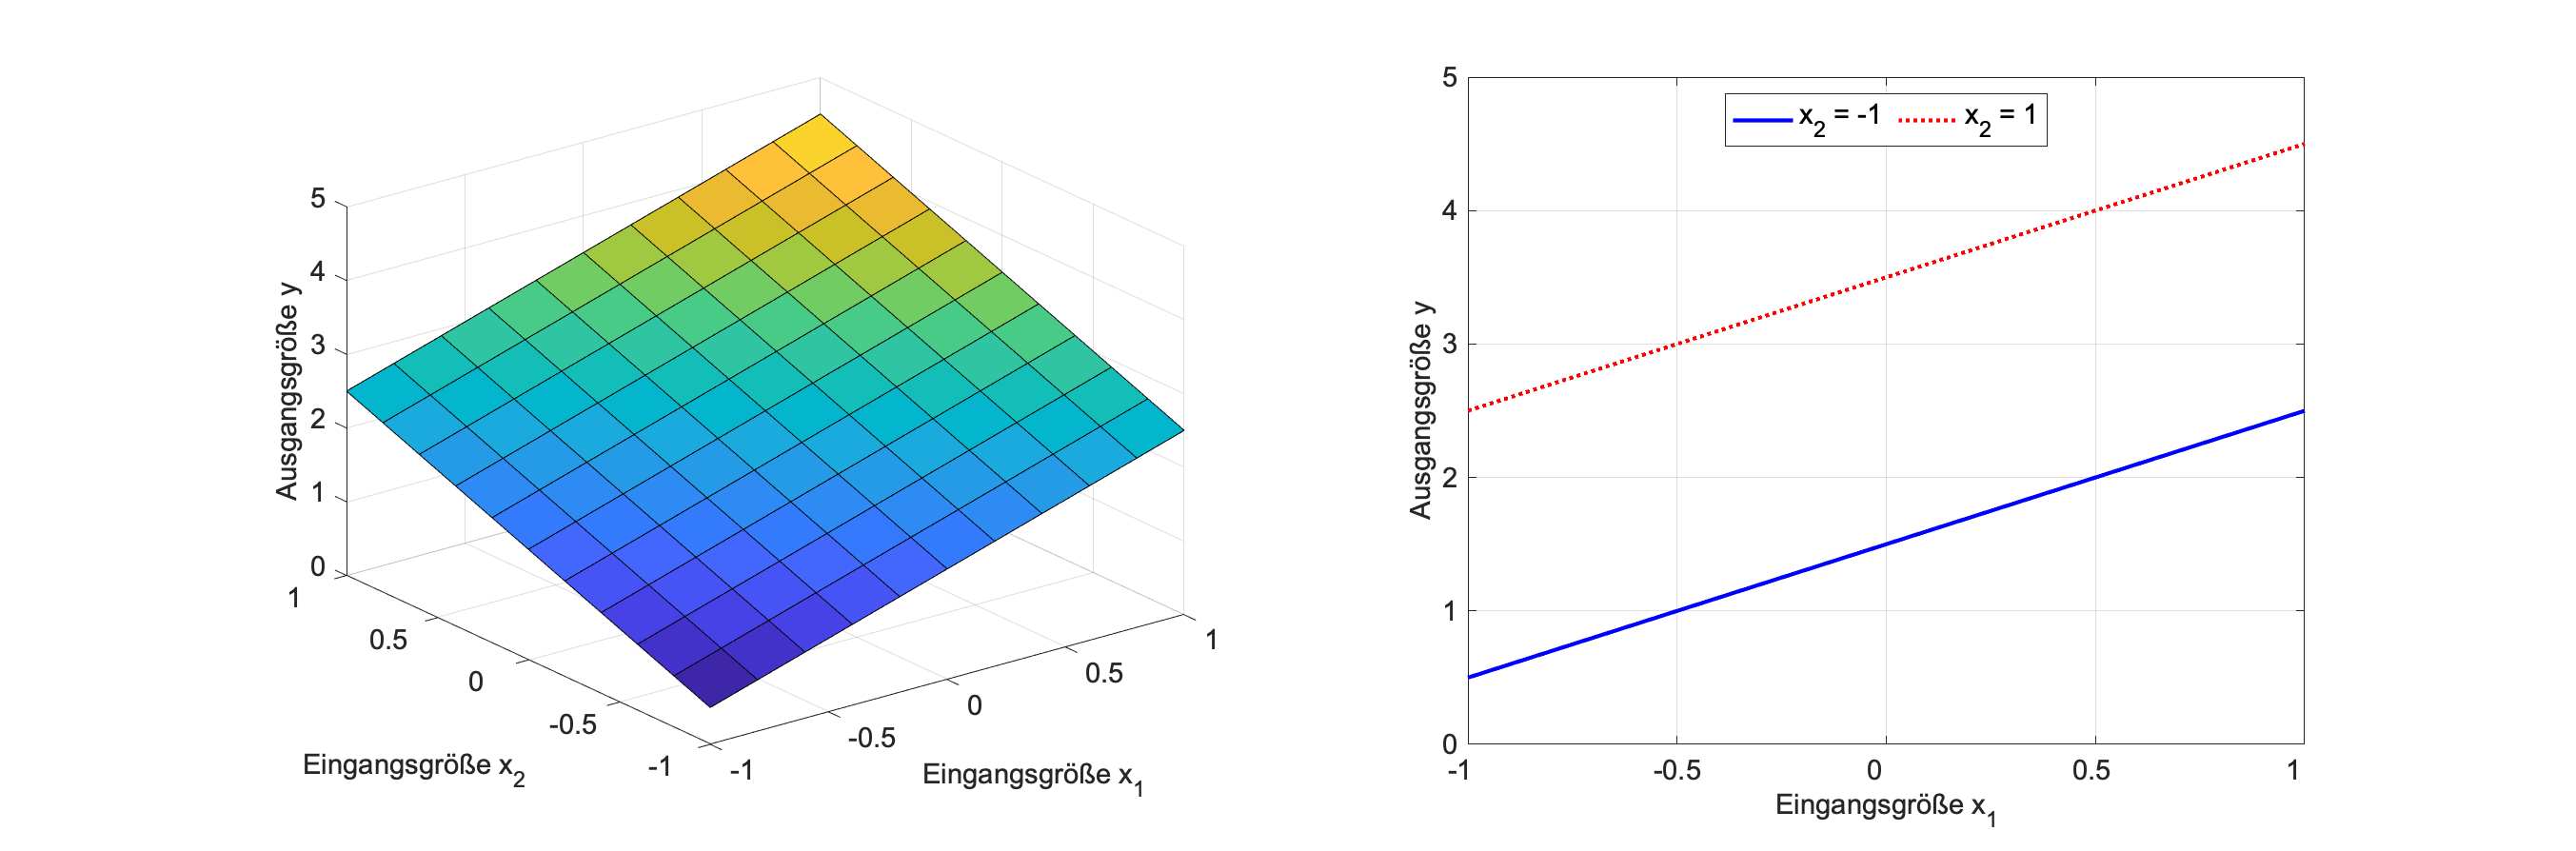
\includegraphics[width=1\textwidth]{Kapitel13/Bilder/image2}}
  \caption{Zielgr\"{o}{\ss}e y f\"{u}r einen linearen Modellansatz}
  \label{fig:Funktionsansatz}
\end{figure}

\noindent Dies wird besonders gut deutlich, wenn die Zielgr\"{o}{\ss}e wie in dem rechten Teil der Darstellung nur als Funktion einer Variablen, hier der Variablen $x_{1}$, dargestellt wird. Die Linien besitzen immer dieselbe Steigung, sie kreuzen sich nicht. Dieses Bild der parallelen Kennlinien ist charakteristisch f\"{u}r lineare Modelle ohne Wechselwirkung. Die linearen Anteile einer Regression werden als Haupteffekte bezeichnet, da sie in vielen Modellen die wesentlichen Abh\"{a}ngigkeiten abdecken.

\clearpage 

\fontfamily{phv}\selectfont
\noindent\textbf{Modellansatz mit Wechselwirkungen} \smallskip

\noindent Funktionen mit Wechselwirkungen sind an einer Sattelfunktion zu erkennen. Die Wirkung der Eingangsgr\"{o}{\ss}en $x_{1}$ ist von der Eingangsgr\"{o}{\ss}e $x_{2}$ abh\"{a}ngig und umgekehrt. Das kann zu einer gegenseitigen Verst\"{a}rkung oder Abschw\"{a}chung f\"{u}hren. Mathematisch Herleitung der Bestimmungsgleichungwerden Wechselwirkungen beschrieben durch den Wechselwirkungsterm

\begin{equation}\label{eq:thirteentwentytwo}
y=b_{0} +b_{3} \cdot x_{1} \cdot x_{2}
\end{equation}

\noindent Bild \ref{fig:Funktionsansatz2} stellt die Zielgr\"{o}{\ss}e y als Funktion der Variablen $x_{1}$ und $x_{2}$ f\"{u}r die Funktion

\begin{equation}\label{eq:thirteentwentythree}
y=2.5+x_{1} \cdot x_{2}
\end{equation}

\noindent dar. 

\noindent 
\begin{figure}[H]
  \centerline{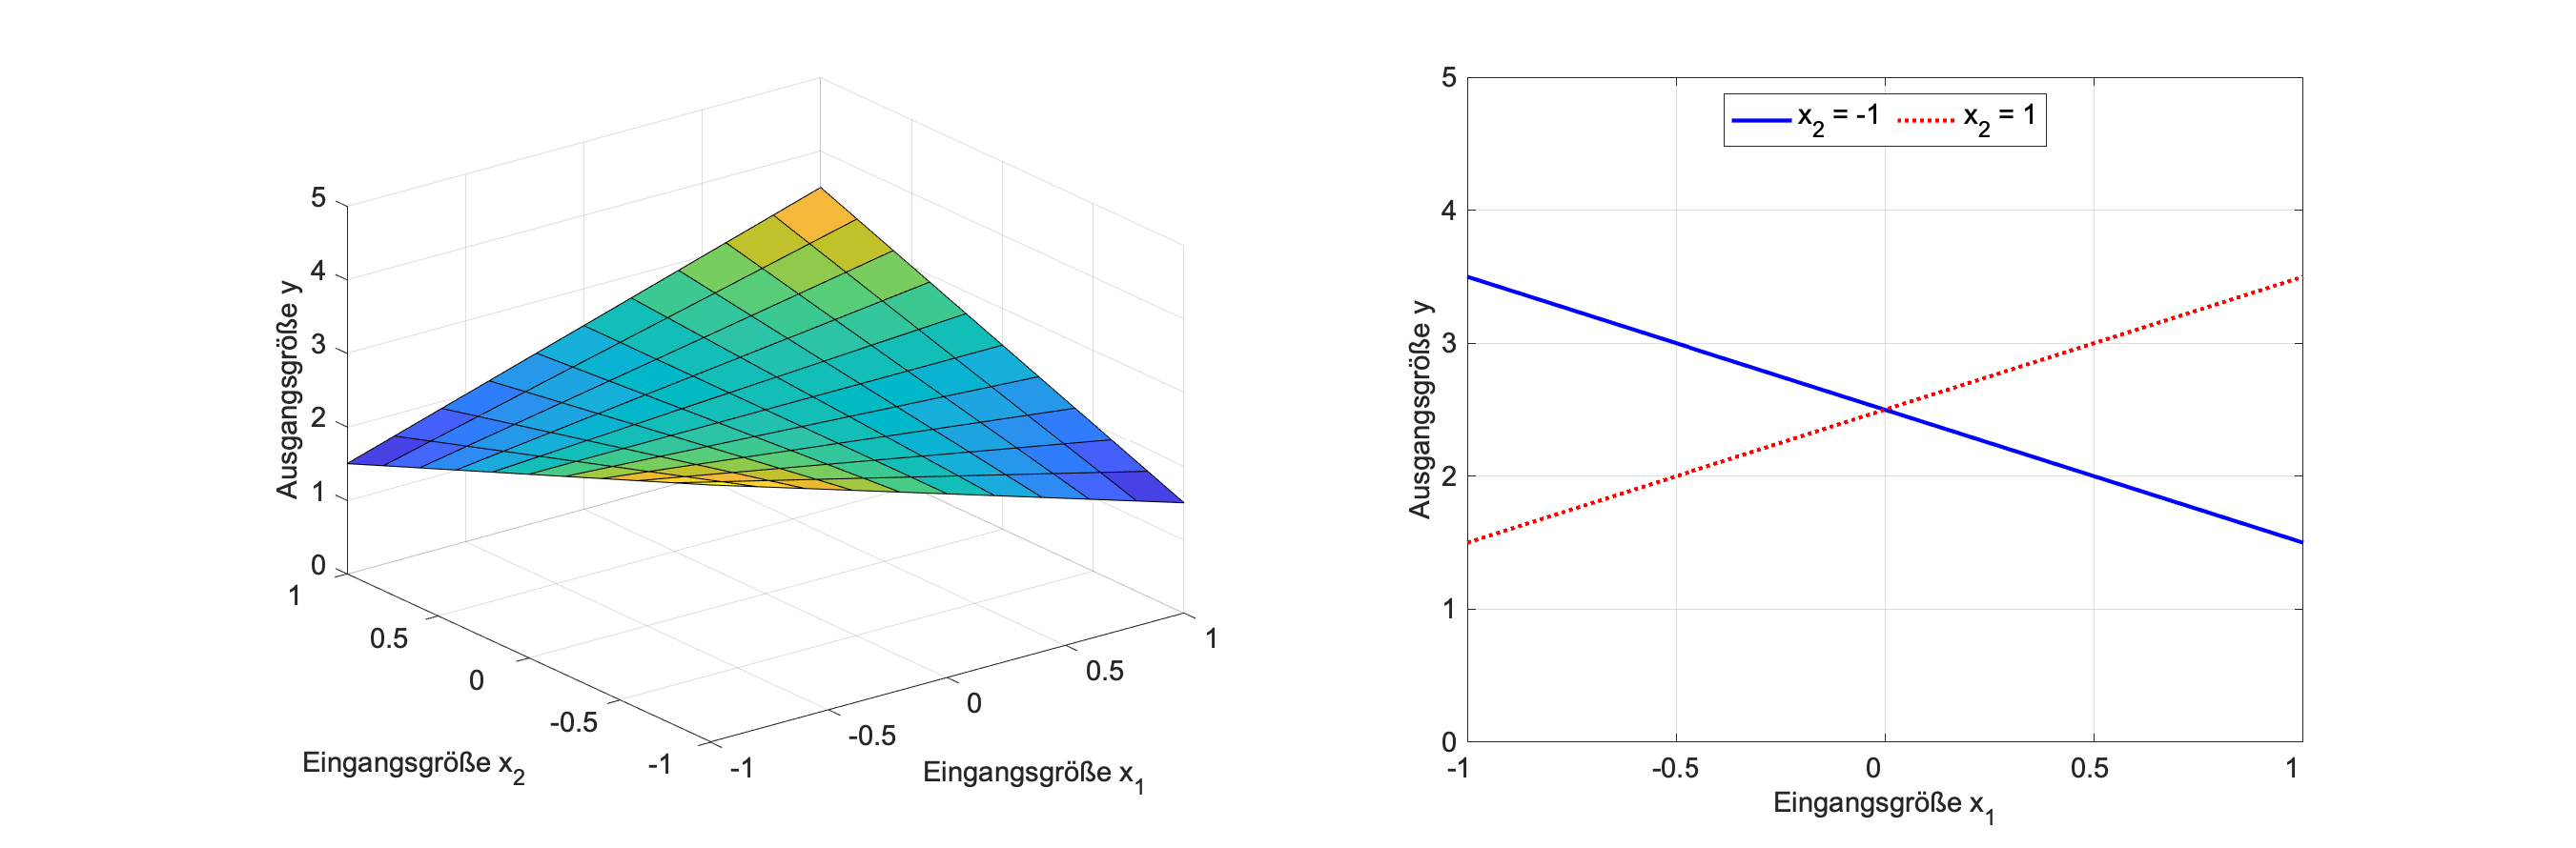
\includegraphics[width=1\textwidth]{Kapitel13/Bilder/image3}}
  \caption{Zielgr\"{o}{\ss}e y f\"{u}r einen Modellansatz mit Wechselwirkungsterm}
  \label{fig:Funktionsansatz2}
\end{figure}

\noindent Die Steigung in Richtung der Variable $x_{1}$ ist von der Variable $x_{2}$ abh\"{a}ngig. Diese Abh\"{a}ngigkeit wird im rechten Teil der Darstellung noch deutlicher. In Abh\"{a}ngigkeit der Variable $x_{2}$ wechselt die Steigung der Gerade $y(x_{1})$ das Vorzeichen.\bigskip

\fontfamily{phv}\selectfont
\noindent\textbf{Quadratischer Modellansatz} \smallskip

\noindent Als letzter Ansatz f\"{u}r eine Regressionsfunktion wird der quadratische Ansatz diskutiert. Er wird mathematisch dargestellt \"{u}ber die Gleichung

\begin{equation}\label{eq:thirteentwentyfour}
y=2.5+b_{4} \cdot x_{1}^{2} +b_{5} \cdot x_{2}^{2}
\end{equation}

\noindent Je nach Vorzeichen der Koeffizienten $b_{4}$ und $b_{5}$ ergeben sich unterschiedliche Topologien. Bild \ref{fig:Funktionsansatz3} zeigt die Zielgr\"{o}{\ss}e f\"{u}r die Funktion

\begin{equation}\label{eq:thirteentwentyfive}
y=2.5+x_{1}^{2} +x_{2}^{2}
\end{equation}

\noindent 
\begin{figure}[H]
  \centerline{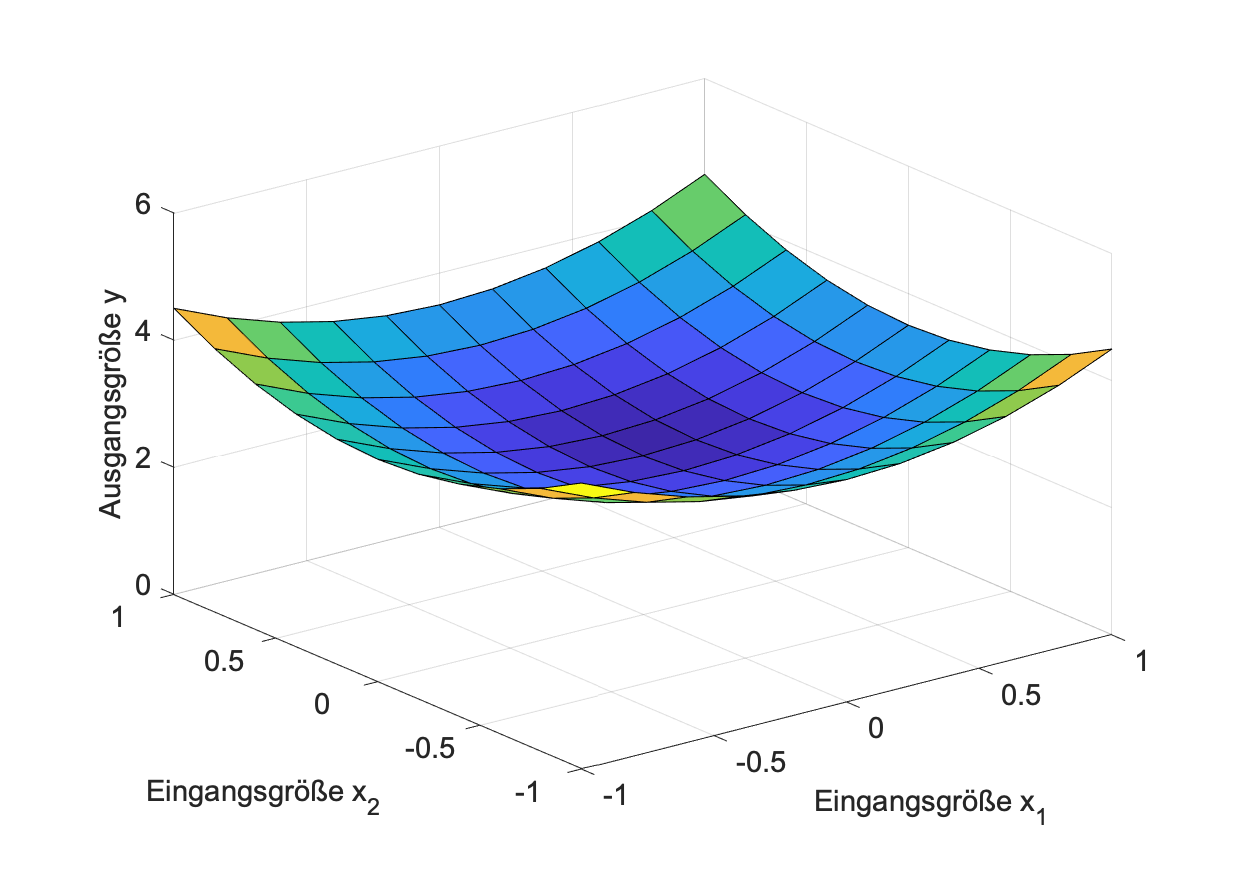
\includegraphics[width=0.5\textwidth]{Kapitel13/Bilder/image4}}
  \caption{Zielgr\"{o}{\ss}e y f\"{u}r einen rein quadratischen Modellansatz bei gleichen Vorzeichen}
  \label{fig:Funktionsansatz3}
\end{figure}

\noindent Weil beide Vorzeichen positiv sind, steigt der Zielgr\"{o}{\ss}e y, sobald sich die Eingangsgr\"{o}{\ss}en aus dem Koordinatenursprung bewegen. Bild 12.5 zeigt eine Fl\"{a}che f\"{u}r die Funktion

\begin{equation}\label{eq:thirteentwentysix}
y=2.5-x_{1}^{2} +x_{2}^{2}
\end{equation}

IMAGE5

\noindent Bild 12.5: Zielgr\"{o}{\ss}e y f\"{u}r einen rein quadratischen Modellansatz bei ungleichen Vorzeichen

\noindent In Richtung steigender Werte f\"{u}r $x_{1}$ wird die Zielgr\"{o}{\ss}e y kleiner, w\"{a}hrend sie f\"{u}r steigende Werte von $x_{2}$ ansteigt. \bigskip

{\fontfamily{phv}\selectfont
\noindent\textbf{Aufbereitung des Datensatzes}} \smallskip

\noindent Zur Berechnung der Regressionsfunktion muss die Datenmatrix \textbf{X} erweitert werden. Durch die elementweise Multiplikation zweier Vektoren \underbar{x}$_{j}$ und \underbar{x}$_{k}$ ensteht ein Vektor\underbar{x}$_{m}$, der Wechselwirkungen der beiden Gr\"{o}{\ss}en rep\"{a}sentiert.

\begin{equation}\label{eq:thirteentwentyseven}
x_{nm} =x_{nj} \cdot x_{nk}
\end{equation}

\noindent F\"{u}r quadratische Regressionsterme wird ein Vektor \underbar{x}$_{k}$ elementweise quadriert. Es entsteht ein neuer Vektor \underbar{x}$_{m}$.

\begin{equation}\label{eq:thirteentwentyeight}
x_{nm} =x_{nk}^{2}
\end{equation}

\clearpage

\noindent
\colorbox{lightgray}{%
\arrayrulecolor{white}%
\renewcommand\arraystretch{0.6}%
\begin{tabular}{ wl{16.5cm} }
{\fontfamily{phv}\selectfont
\noindent{Beispiel: Feuchtesensor}}
\end{tabular}%
}\bigskip

\noindent Als Beispiel f\"{u}r eine multivariate Regression mit vollquadratischem Ansatz wird die Vermessung der Kapazit\"{a}t eines Feuchtesensors betrachtet. Die aufgenommenen Messergebnisse zeigt Tabelle \ref{tab:thirteentwo}. Die Kapazit\"{a}t des Feuchtesensors soll mit einer Regressionsfunktion beschrieben werden. Eingangsgr\"{o}{\ss}en sind die relative Feuchte rF und die Temperatur T, Zielgr\"{o}{\ss}e ist die Sensorkapazit\"{a}t $C_{P}$.

\begin{equation}\label{eq:thirteentwentynine}
y=C_{P} =f(rF,T)
\end{equation}

\begin{table}[H]
\setlength{\arrayrulewidth}{.1em}
\caption{Urliste einer Vermessung von Feuchtesensoren}
\setlength{\fboxsep}{0pt}%
\colorbox{lightgray}{%
\arrayrulecolor{white}%
\begin{tabular}{ wc{1.2cm} | wc{1.8cm} | wc{1.8cm} | wc{1.9cm} | wc{1.9cm} | wc{1.8cm} | wc{1.8cm} | wc{1.8cm}}
\hline\xrowht{7pt}

\multirow{3}{*}{\fontfamily{phv}\selectfont\textbf{Nr.}} &
\multirow{2}{*}{\fontfamily{phv}\selectfont\textbf{Kapazität}} &
\fontfamily{phv}\selectfont\textbf{Einfügen} &
\fontfamily{phv}\selectfont\textbf{Temperatur} &
\fontfamily{phv}\selectfont\textbf{rel. Feuchte} &
\multicolumn{3}{c}{\fontfamily{phv}\selectfont\textbf{Neu generierte Datenspalten}} \\  \xrowht{7pt}

& 
\multirow{2.5}{*}{\fontfamily{phv}\selectfont\textbf{C$_{\textbf{p}}$ pF}} & 
\fontfamily{phv}\selectfont\textbf{Konstante} & 
\fontfamily{phv}\selectfont\textbf{T / $^{\circ}$C} & 
\fontfamily{phv}\selectfont\textbf{rF / \%} & 
\multicolumn{3}{c}{\fontfamily{phv}\selectfont\textbf{für vollquadratischen Ansatz}} \\ \cline{3-8} \xrowht{7pt}

&
&
\fontfamily{phv}\selectfont{1} &
\fontfamily{phv}\selectfont{x$_{1}$} &
\fontfamily{phv}\selectfont{x$_{2}$} &
\fontfamily{phv}\selectfont{x$_{1}\cdot $ x$_{2} $} &
\fontfamily{phv}\selectfont{x$_{1}^{2}$} &
\fontfamily{phv}\selectfont{x$_{2}^{2}$} \\ \hline \xrowht{10pt}

\fontfamily{phv}\selectfont{1} &
\fontfamily{phv}\selectfont{179.3} &
\fontfamily{phv}\selectfont{1} &
\fontfamily{phv}\selectfont{90.0} &
\fontfamily{phv}\selectfont{9.5} &
\fontfamily{phv}\selectfont{855} &
\fontfamily{phv}\selectfont{8100} &
\fontfamily{phv}\selectfont{90.25} \\ \hline \xrowht{10pt}

\fontfamily{phv}\selectfont{2} &
\fontfamily{phv}\selectfont{182.6} &
\fontfamily{phv}\selectfont{1} &
\fontfamily{phv}\selectfont{90.0} &
\fontfamily{phv}\selectfont{19.8} &
\fontfamily{phv}\selectfont{1782} &
\fontfamily{phv}\selectfont{8100} &
\fontfamily{phv}\selectfont{392.04} \\ \hline \xrowht{10pt}

\fontfamily{phv}\selectfont{3} &
\fontfamily{phv}\selectfont{182.6} &
\fontfamily{phv}\selectfont{1} &
\fontfamily{phv}\selectfont{44.9} &
\fontfamily{phv}\selectfont{17.8} &
\fontfamily{phv}\selectfont{799.22} &
\fontfamily{phv}\selectfont{2016.01} &
\fontfamily{phv}\selectfont{316.84} \\ \hline \xrowht{10pt}

\fontfamily{phv}\selectfont{4} &
\fontfamily{phv}\selectfont{185.6} &
\fontfamily{phv}\selectfont{1} &
\fontfamily{phv}\selectfont{90.1} &
\fontfamily{phv}\selectfont{29.6} &
\fontfamily{phv}\selectfont{2666.96} &
\fontfamily{phv}\selectfont{8118.01} &
\fontfamily{phv}\selectfont{876.16} \\ \hline \xrowht{10pt}

\fontfamily{phv}\selectfont{5} &
\fontfamily{phv}\selectfont{185.6} &
\fontfamily{phv}\selectfont{1} &
\fontfamily{phv}\selectfont{45.2} &
\fontfamily{phv}\selectfont{27.2} &
\fontfamily{phv}\selectfont{1229.44} &
\fontfamily{phv}\selectfont{2043.04} &
\fontfamily{phv}\selectfont{739.84} \\ \hline \xrowht{10pt}

\fontfamily{phv}\selectfont{6} &
\fontfamily{phv}\selectfont{189.8} &
\fontfamily{phv}\selectfont{1} &
\fontfamily{phv}\selectfont{89.7} &
\fontfamily{phv}\selectfont{40.6} &
\fontfamily{phv}\selectfont{3641.82} &
\fontfamily{phv}\selectfont{8046.09} &
\fontfamily{phv}\selectfont{1648.36} \\ \hline \xrowht{10pt}

\fontfamily{phv}\selectfont{7} &
\fontfamily{phv}\selectfont{189.0} &
\fontfamily{phv}\selectfont{1} &
\fontfamily{phv}\selectfont{45.6} &
\fontfamily{phv}\selectfont{36.8} &
\fontfamily{phv}\selectfont{1678.08} &
\fontfamily{phv}\selectfont{2079.36} &
\fontfamily{phv}\selectfont{1354.24} \\ \hline \xrowht{10pt}

\fontfamily{phv}\selectfont{8} &
\fontfamily{phv}\selectfont{188.2} &
\fontfamily{phv}\selectfont{1} &
\fontfamily{phv}\selectfont{22.8} &
\fontfamily{phv}\selectfont{36.7} &
\fontfamily{phv}\selectfont{836.76} &
\fontfamily{phv}\selectfont{519.84} &
\fontfamily{phv}\selectfont{1346.89} \\ \hline \xrowht{10pt}

\fontfamily{phv}\selectfont{9} &
\fontfamily{phv}\selectfont{192.6} &
\fontfamily{phv}\selectfont{1} &
\fontfamily{phv}\selectfont{89.6} &
\fontfamily{phv}\selectfont{50.1} &
\fontfamily{phv}\selectfont{4488.96} &
\fontfamily{phv}\selectfont{8028.16} &
\fontfamily{phv}\selectfont{2510.01} \\ \hline \xrowht{10pt}

\fontfamily{phv}\selectfont{10} &
\fontfamily{phv}\selectfont{192.1} &
\fontfamily{phv}\selectfont{1} &
\fontfamily{phv}\selectfont{45.3} &
\fontfamily{phv}\selectfont{47.4} &
\fontfamily{phv}\selectfont{2147.22} &
\fontfamily{phv}\selectfont{2052.09} &
\fontfamily{phv}\selectfont{2246.76} \\ \hline \xrowht{10pt}

\fontfamily{phv}\selectfont{11} &
\fontfamily{phv}\selectfont{190.9} &
\fontfamily{phv}\selectfont{1} &
\fontfamily{phv}\selectfont{22.7} &
\fontfamily{phv}\selectfont{46.4} &
\fontfamily{phv}\selectfont{1053.28} &
\fontfamily{phv}\selectfont{515.29} &
\fontfamily{phv}\selectfont{2152.96} \\ \hline \xrowht{10pt}

\fontfamily{phv}\selectfont{12} &
\fontfamily{phv}\selectfont{194.6} &
\fontfamily{phv}\selectfont{1} &
\fontfamily{phv}\selectfont{90.0} &
\fontfamily{phv}\selectfont{60.2} &
\fontfamily{phv}\selectfont{5418} &
\fontfamily{phv}\selectfont{8100} &
\fontfamily{phv}\selectfont{3624.04} \\ \hline \xrowht{10pt}

\fontfamily{phv}\selectfont{13} &
\fontfamily{phv}\selectfont{195.2} &
\fontfamily{phv}\selectfont{1} &
\fontfamily{phv}\selectfont{45.2} &
\fontfamily{phv}\selectfont{57.8} &
\fontfamily{phv}\selectfont{2612.56} &
\fontfamily{phv}\selectfont{2043.04} &
\fontfamily{phv}\selectfont{3340.84} \\ \hline \xrowht{10pt}

\fontfamily{phv}\selectfont{14} &
\fontfamily{phv}\selectfont{194.5} &
\fontfamily{phv}\selectfont{1} &
\fontfamily{phv}\selectfont{22.6} &
\fontfamily{phv}\selectfont{57.7} &
\fontfamily{phv}\selectfont{1304.02} &
\fontfamily{phv}\selectfont{510.76} &
\fontfamily{phv}\selectfont{3329.29} \\ \hline \xrowht{10pt}

\fontfamily{phv}\selectfont{15} &
\fontfamily{phv}\selectfont{197.8} &
\fontfamily{phv}\selectfont{1} &
\fontfamily{phv}\selectfont{90.0} &
\fontfamily{phv}\selectfont{70.3} &
\fontfamily{phv}\selectfont{6327} &
\fontfamily{phv}\selectfont{8100} &
\fontfamily{phv}\selectfont{4942.09} \\ \hline \xrowht{10pt}

\fontfamily{phv}\selectfont{16} &
\fontfamily{phv}\selectfont{198.6} &
\fontfamily{phv}\selectfont{1} &
\fontfamily{phv}\selectfont{45.2} &
\fontfamily{phv}\selectfont{68.5} &
\fontfamily{phv}\selectfont{3096.2} &
\fontfamily{phv}\selectfont{2043.04} &
\fontfamily{phv}\selectfont{4692.25} \\ \hline \xrowht{10pt}

\fontfamily{phv}\selectfont{17} &
\fontfamily{phv}\selectfont{198.2} &
\fontfamily{phv}\selectfont{1} &
\fontfamily{phv}\selectfont{22.8} &
\fontfamily{phv}\selectfont{69.1} &
\fontfamily{phv}\selectfont{1575.48} &
\fontfamily{phv}\selectfont{519.84} &
\fontfamily{phv}\selectfont{4774.81} \\ \hline \xrowht{10pt}

\fontfamily{phv}\selectfont{18} &
\fontfamily{phv}\selectfont{201.6} &
\fontfamily{phv}\selectfont{1} &
\fontfamily{phv}\selectfont{89.9} &
\fontfamily{phv}\selectfont{80.1} &
\fontfamily{phv}\selectfont{7200.99} &
\fontfamily{phv}\selectfont{8082.01} &
\fontfamily{phv}\selectfont{6416.01} \\ \hline \xrowht{10pt}

\fontfamily{phv}\selectfont{19} &
\fontfamily{phv}\selectfont{202.6} &
\fontfamily{phv}\selectfont{1} &
\fontfamily{phv}\selectfont{45.2} &
\fontfamily{phv}\selectfont{79.5} &
\fontfamily{phv}\selectfont{3593.4} &
\fontfamily{phv}\selectfont{2043.04} &
\fontfamily{phv}\selectfont{6320.25} \\ \hline \xrowht{10pt}

\fontfamily{phv}\selectfont{20} &
\fontfamily{phv}\selectfont{201.2} &
\fontfamily{phv}\selectfont{1} &
\fontfamily{phv}\selectfont{22.8} &
\fontfamily{phv}\selectfont{78.6} &
\fontfamily{phv}\selectfont{1792.08} &
\fontfamily{phv}\selectfont{519.84} &
\fontfamily{phv}\selectfont{6177.96} \\ \hline \xrowht{10pt}

\fontfamily{phv}\selectfont{21} &
\fontfamily{phv}\selectfont{201.5} &
\fontfamily{phv}\selectfont{1} &
\fontfamily{phv}\selectfont{9.6} &
\fontfamily{phv}\selectfont{75.9} &
\fontfamily{phv}\selectfont{728.64} &
\fontfamily{phv}\selectfont{92.16} &
\fontfamily{phv}\selectfont{5760.81} \\ \hline

\end{tabular}%
}
\label{tab:thirteentwo}
\end{table}

\noindent Um sich einen Eindruck \"{u}ber die Daten zu verschaffen, werden die St\"{u}tzstellen, an denen die Werte aufgenommen wurden, in einer Ebene aus relativer Feuchte und Temperatur in Bild 12.6 grafisch dargestellt.

IMAGE6

\noindent Bild 12.6: Darstellung der St\"{u}tzstellen, an denen die Messwerte f\"{u}r die Kapazit\"{a}t $C_{p}$ eines Feuchtesensors gemessen wurde

\noindent Der Bereich geringer relativer Feuchte rF und kleiner Temperaturen T wurde bei der Messung ausgespart, da das eingesetzte Messger\"{a}t in diesem Bereich keine ausreichende Messf\"{a}higkeit aufweist. Bild 12.7Bild 12.7 stellt die einzelnen Messwerte als dreidimensionales Streudiagramm dar.

IMAGE7

\noindent Bild 12.7: Kapazit\"{a}t C${}_{p}$ eines Feuchtesensors als Funktion der Temperatur Tund relativen Feuchte rF als Streudiagramm

\noindent Die Daten weisen ein weitgehend lineares Verhalten auf. Die Kapazit\"{a}t steigt in Richtung hoher Feuchte an. Das vollquadratische Modell wird angesetzt, um Linearit\"{a}tsfehler bewerten zu k\"{o}nnen. Dazu wird jede Variable bis zur zweiten Potenz sowie die einfache Wechselwirkung zwischen relativer Feuchte und Temperatur ber\"{u}cksichtigt. Dadurch ergibt sich als Vektor der Eingangsgr\"{o}{\ss}en zu

\begin{equation}\label{eq:thirteenthirty}
\underline{x}_{n}^{T} =\left(1 rF_{n} T_{n} rF_{n} \cdot T_{n} rF_{n}^{2} T_{n}^{2} \right)
\end{equation}

\noindent Die dabei entstehende Erweiterung der Datenmatrix ist in Tabelle 12.2 bereits eingetragen. Mit dem Datensatz wird die Regressionsgleichung berechnet. F\"{u}r die Koeffizienten $b_{m}$ ergibt sich der Vektor

\begin{equation}\label{eq:thirteenthirtyone}
\underline{b}=\left(\textbf{X}^{T} \cdot \textbf{X}\right)^{-1} \cdot \textbf{X}^{T} \cdot \underline{y}=\left(\begin{array}{c} {175.2} \\ {0.327} \\ {0.059} \\ {-0.246\cdot 10^{-3}} \\ {0.015\cdot 10^{-3}} \\ {-0.476\cdot 10^{-3}} \end{array}\right)
\end{equation}

\noindent Die Regressionsgleichung lautet damit

\begin{equation}\label{eq:thirteenthirtytwo}
C_{P} =175.2+0.327\cdot rF+ 0.059\cdot T-0.246\cdot 10^{-3} \cdot rF\cdot T+0.015\cdot 10^{-3} \cdot rF^{2} -0.476\cdot 10^{-3} \cdot T^{2}
\end{equation}

\noindent Das Regressionsergebnis ist in Bild 12.8 f\"{u}r den Temperaturbereich von $10 \dots90 ^{\circ} C$ und den Feuchtebereich von $10 \dots 90 \% rF$ dargestellt.

IMAGE8

\noindent Bild 12.8: Darstellung des Ergebnisses der Regression f\"{u}r einen Temperaturbereich von $10 \dots90 ^{\circ} C$ und einen Feuchtebereich von $10 \dots 90 \% rF$

\subsubsection{L\"{o}sbarkeit }

\noindent $<<<$ Wird sp\"{a}ter erg\"{a}nzt {\dots}

\begin{itemize}
    \item Regression kann mit einer Taylorreihe verglichen werden
    \item Koeffizient vor quadratischem Term ist zweite Ableitung, f''$\cdot\Delta x^{2}$, deshalb muss zweite Ableitung f\"{u}r ein Minimum $ > 0$ sein
    \item Umsetzung im mehrdimensionalen Fall f\"{u}hrt zur sogenannten Hesse-Matrix, sie muss eine Bedingung \"{a}hnlich wie im eindimensionalen Fall erf\"{u}llen: Hesse-Matrix muss positiv definit sein
    \item Kriterium ist aber eher theoretischer Natur, weil die Funktion an sich nicht bekannt ist {\dots}
    \item  Konkrete Bewertungen \"{u}ber Kondition der Matrix = Korrektheit der Regression
\end{itemize}

\noindent $>>>$

\clearpage

\subsection{Statistische Bewertung der Regressionsparameter}

\noindent Die Sch\"{a}tzung der Regressionsparametern $\beta_{m}$ mit den Parametern $b_{m}$ basiert auf den Messwerten $y_{n}$. Sie weisen einen zuf\"{a}lligen Messfehler auf und sind damit Zufallsgr\"{o}{\ss}en. Aus diesem Grund sind auch die mit den Messwerten bestimmten Parameter $b_{m}$ Zufallsgr\"{o}{\ss}en. 

\subsubsection{Modell zur statistischen Bewertung der Regression}

\noindent Die statistische Bewertung beruht auf dem Modellansatz in Gleichung \eqref{eq:thirteenone}. Er kann in Vektorschreibweise dargestellt werden als 

\begin{equation}\label{eq:thirteenthirtythree}
\underline{y}=X\cdot \underline{\beta }+\underline{e}
\end{equation}

\noindent Die Messwerte unterliegen einem Messfehler e. Es wird davon ausgegangen, dass der Messfehler normalverteilt ist. Er weist einen Erwartungswert von 

\begin{equation}\label{eq:thirteenthirtyfour}
E\left(\underline{y}-\underline{\mu }_{y} \right)=E\left(\underline{e}\right)=\underline{0}
\end{equation}

\noindent und eine Kovarianzmatrix von

\begin{equation}\label{eq:thirteenthirtyfive}
E\left(\left(\underline{y}-\underline{\mu }_{y} \right)\cdot \left(\underline{y}-\underline{\mu }_{y} \right)^{T} \right)=E\left(\underline{e}\cdot \underline{e}^{T} \right)=I\cdot \sigma ^{2}
\end{equation}

\noindent Dabei ist \textbf{I} die Einheitsmarix, die nur auf der Hauptdiagonalen Einsen besitzt, alle anderen Werte sind null. Das bedeutet, dass der Messfehler bei allen Messungen konstante Varianz $\sigma^{2}$ besitzt. Alle Kovarianzen $\sigma_{jk}$ sind null, die Messfehler sind voneinander unabh\"{a}ngig. \newline

\noindent Zum Nachweis der Erwartungstreue werden die Erwartungswerte der Regressionsparameter berechnet. 

\begin{equation}\label{eq:thirteenthirtysix}
\begin{split}
E\left(\underline{b}\right) & =E\left(\left(X^{T} \cdot X\right)^{-1} \cdot X^{T} \cdot \underline{y}\right)=E\left(\left(X^{T} \cdot X\right)^{-1} \cdot X^{T} \cdot X\cdot \underline{\beta }+\underline{e}\right) \\ 
& = E\left(\underline{\beta }\right)+\left(X^{T} \cdot X\right)^{-1} \cdot X^{T} \cdot E\left(\underline{e}\right)=\underline{\beta }
\end{split}
\end{equation}

\noindent Die Sch\"{a}tzung ist demnach erwartungstreu. Die Kovarianzmatrix berechnet sich mit der Matrix

\begin{equation}\label{eq:thirteenthirtyseven}
C=\left(X^{T} \cdot X\right)^{-1} \cdot X^{T}
\end{equation}

\noindent zu

\begin{equation}\label{eq:thirteenthirtyeight}
\begin{split}
E\left(\left(\underline{b}-\underline{\beta }\right)\cdot \left(\underline{b}-\underline{\beta }\right)^{T} \right) & =E\left(\left(C\cdot \underline{y}-C\cdot \underline{\mu }_{y} \right)\cdot \left(C\cdot \underline{y}-C\cdot \underline{\mu }_{y} \right)^{T} \right) \\ 
& = C\cdot E\left(\left(\underline{y}-\underline{\mu }_{y} \right)\cdot \left(\underline{y}-\underline{\mu }_{y} \right)^{T} \right)\cdot C^{T} =C\cdot I\cdot \sigma ^{2} \cdot C^{T} =C\cdot C^{T} \cdot \sigma ^{2}
\end{split}
\end{equation}

\noindent Die Streuung der Koeffizienten ist demnach proportional zur Streuung der Messung. Durch Einsetzen von Gleichung \eqref{eq:thirteenthirtyseven} ergibt sich wegen 

\begin{equation}\label{eq:thirteenthirtynine}
C\cdot C^{T} =\left(\left(X^{T} \cdot X\right)^{-1} \cdot X^{T} \right)\cdot \left(\left(X^{T} \cdot X\right)^{-1} \cdot X^{T} \right)^{T} =\left(X^{T} \cdot X\right)^{-1} \cdot X^{T} \cdot X\cdot \left(X^{T} \cdot X\right)^{-1} =\left(X^{T} \cdot X\right)^{-1}
\end{equation}

\noindent der Ausdruck f\"{u}r die Kovarianzmatrix der Regressionsparameter

\begin{equation}\label{eq:thirteenfourty}
E\left(\left(\underline{b}-\underline{\beta }\right)\cdot \left(\underline{b}-\underline{\beta }\right)^{T} \right)=C\cdot C^{T} \cdot \sigma ^{2} =\left(X^{T} \cdot X\right)^{-1} \cdot \sigma ^{2}
\end{equation}

\noindent Dabei ist die Varianz der Messung $\sigma^{2}$ unbekannt und muss ebenfalls gesch\"{a}tzt werden. Die Absch\"{a}tzung erfolgt \"{u}ber die Summe der Fehlerquadrate als Stichprobenvarianz. Aus N Messungen sind M + 1 Parameter zu bestimmen. Damit liegen N - M - 1 Freiheitsgrade vor, und die Stichprobenvarianz berechnet sich zu

\begin{equation}\label{eq:thirteenfourtyone}
\begin{split}
\sigma ^{2} \approx s^{2}  & =\frac{1}{N-M-1} \cdot \sum _{n=1}^{N}r_{n}^{2}  =\frac{1}{N-M-1} \cdot \left(\underline{y}-X\cdot \underline{b}\right)^{T} \cdot \left(\underline{y}-X\cdot \underline{b}\right) \\ 
& = \frac{1}{N-M-1} \cdot \left(\underline{y}^{T} -\underline{b}^{T} \cdot X^{T} \right)\cdot \left(\underline{y}-X\cdot \underline{b}\right) \\
& = \frac{1}{N-M-1} \cdot \left(\underline{y}^{T} \cdot \underline{y}-\underline{y}^{T} \cdot X\cdot \underline{b}-\underline{b}^{T} \cdot X^{T} \cdot \underline{y}+\underline{b}^{T} \cdot X^{T} \cdot X\cdot \underline{b}\right) \\
& = \frac{1}{N-M-1} \cdot \left(\underline{y}^{T} \cdot \underline{y}-\underline{y}^{T} \cdot X\cdot \underline{b}-\underline{b}^{T} \cdot X^{T} \cdot \left(\underline{y}-X\cdot \underline{b}\right)\right) \\ 
& = \frac{1}{N-M-1} \cdot \left(\underline{y}^{T} \cdot \underline{y}-\underline{y}^{T} \cdot X\cdot \underline{b}\right)
\end{split}
\end{equation}

\noindent Die Summanden in der Klammer sind skalare Gr\"{o}{\ss}en. Damit gilt

\begin{equation}\label{eq:thirteenfourtytwo}
\underline{y}^{T} \cdot X\cdot \underline{b}=\underline{b}^{T} \cdot X^{T} \cdot \underline{y}
\end{equation}

\noindent und die Varianz der Messgr\"{o}{\ss}e kann abgesch\"{a}tzt werden mit

\begin{equation}\label{eq:thirteenfourtythree}
\sigma ^{2} \approx s^{2} =\frac{1}{N-M-1} \cdot \left(\underline{y}^{T} \cdot \underline{y}-\underline{b}^{T} \cdot X^{T} \cdot \underline{y}\right)
\end{equation}

\subsubsection{Bewertung der Regressionsparameter $b_{m}$}

\noindent Mit den Vor\"{u}berlegungen in Abschnitt 12.2.1 zur Kovarianzmatrix und zur Varianz der Messgr\"{o}{\ss}e k\"{o}nnen zur Bewertung der Regressionskoeffizienten $b_{m}$ Zufallsvariablen aufgebaut werden. Mit $k_{m}^{2}$ als Element (m,m) der Matrix $(\textbf{X}^{T}\cdot \textbf{X})^{-1}$ sind die Zufallsvariablen

\begin{equation}\label{eq:thirteenfourtyfour}
t_{m} =\frac{b_{m} -\beta _{m} }{k_{m} \cdot s}
\end{equation}

\noindent t-verteilt mit N - M - 1 Freiheitsgraden. Die Zufallsvariablen t werden genutzt, um den Konfidenzbereich abzusch\"{a}tzen und die Signifikanz zu bewerten.\bigskip

{\fontfamily{phv}\selectfont
\noindent\textbf{Konfidenzintervall f\"{u}r die Regressionskoeffizienten $\beta_{m}$}} \smallskip

\noindent Zur Berechnung des Konfidenzintervalls des Regressionskoeffizienten $\beta_{m}$ wird die Zufallsvariable $t_{m}$ verwendet. Nach den Ausf\"{u}hrungen in Kapitel 5 berechnet sich der Konfidenzbereich aus der Wahrscheinlichkeit

\begin{equation}\label{eq:thirteenfourtyfive}
P(c_{1} <t_{m} \le c_{2})=F(c_{2})-F(c_{1})=\gamma
\end{equation}

\noindent Durch die Symmetrie des Konfidenzbereichs ergeben sich die Konstanten $c_{1}$ und $c_{2}$ zu

\begin{equation}\label{eq:thirteenfourtysix}
c_{1} =F^{-1} \left(\frac{1-\gamma }{2} \right)
\end{equation}

\noindent und

\begin{equation}\label{eq:thirteenfourtyseven}
c_{2} =F^{-1} \left(\frac{1+\gamma }{2} \right)
\end{equation}

\noindent Durch Umformungen von Gleichung \eqref{eq:thirteenfourtyone} ergibt sich ein Ausdruck f\"{u}r den Konfidenzbereich des Regressionskoeffizienten $\beta_{m}$ von

\begin{equation}\label{eq:thirteenfourtyeight}
\gamma =P\left(c_{1} <t_{m} \le c_{2} \right)=P\left(c_{1} <\frac{b_{m} -\beta _{m} }{k_{m} \cdot s} \le c_{2} \right)=P\left(b_{m} -c_{2} \cdot k_{m} \cdot s\le \beta _{m} <b_{m} -c_{1} \cdot k_{m} \cdot s\right)
\end{equation}

\noindent Die Berechnung wird in Tabelle \ref{tab:thirteenthree} zusammengefasst.

\begin{table}[H]
\setlength{\arrayrulewidth}{.1em}
\caption{Vorgehen zur Bestimmung des Konfidenzbereichs f\"{u}r den Regressionskoeffizienten $\beta_{m}$}
\setlength{\fboxsep}{0pt}%
\colorbox{lightgray}{%
\arrayrulecolor{white}%
\begin{tabular}{| wc{2.6cm} | wc{14cm} }
\xrowht{15pt}

\fontfamily{phv}\selectfont\textbf{Nr.} & 
\fontfamily{phv}\selectfont\textbf{Prozessschritt}\\ \hline \xrowht{20pt}

\fontfamily{phv}\selectfont{1} &
\fontfamily{phv}\selectfont{Wahl einer Konfidenzzahl $\gamma$}\\ \hline \xrowht{10pt}

\multirow{4}{*}{\fontfamily{phv}\selectfont{2}} &
\fontfamily{phv}\selectfont{Bestimmung der zugehörigen Parameter c$_{1}$ und c$_{2}$ aus der inversen} \\ \xrowht{10pt}
& \fontfamily{phv}\selectfont{t-Verteilung mit N + M – 1 Freiheitsgraden}  \\\xrowht{25pt}
& \fontfamily{phv}\selectfont{$c_{1} =F^{-1} \left(\frac{1-\gamma }{2} \right)\qquad $  und  $\qquad c_{2} =F^{-1} \left(\frac{1+\gamma }{2} \right)$}  \\ \hline
\xrowht{10pt}

\multirow{3}{*}{\fontfamily{phv}\selectfont{3}} &
\fontfamily{phv}\selectfont{Berechnung der Regressonskoeffizienten}\\ \xrowht{20pt}

&
\fontfamily{phv}\selectfont{$\underline{b}=\left(X^{T} \cdot X\right)^{-1} \cdot X^{T} \cdot \underline{y}$}\\\hline \xrowht{10pt}

\multirow{5}{*}{\fontfamily{phv}\selectfont{4}} &
\fontfamily{phv}\selectfont{Absch\"{a}tzung der Kovarianzmatrix}\\ \xrowht{20pt}

&
\fontfamily{phv}\selectfont{$\left(X^{T} \cdot X\right)^{-1} \cdot \frac{1}{N-M-1} \cdot \left(\underline{y}^{T} \cdot \underline{y}-\underline{b}^{T} \cdot X^{T} \cdot \underline{y}\right)=\left(\begin{array}{ccc} {k_{1} } & {\cdots } & {0} \\ {\vdots } & {\ddots } & {\vdots } \\ {0} & {\cdots } & {k_{M} } \end{array}\right)$}\\\hline \xrowht{10pt}

\multirow{3}{*}{\fontfamily{phv}\selectfont{5}} &
\fontfamily{phv}\selectfont{Bestimmung des Konfidenzintervalls}\\ \xrowht{20pt}

&
\fontfamily{phv}\selectfont{$b_{m} -c_{2} \cdot k_{m} \cdot s\le \beta _{m} <b_{m} -c_{1} \cdot k_{m} \cdot s$}\\\hline 

\end{tabular}%
}\bigskip
\label{tab:thirteenthree}
\end{table}

\clearpage

\noindent
\colorbox{lightgray}{%
\arrayrulecolor{white}%
\renewcommand\arraystretch{0.6}%
\begin{tabular}{ wl{16.5cm} }
{\fontfamily{phv}\selectfont
\noindent{Beispiel: Feuchtesensor}}
\end{tabular}%
}\bigskip

\noindent Die Berechnung der Konfidenzbereiche wird an dem Beispiel des Feuchtesensors angewendet. F\"{u}r die Koeffizienten $b_{m}$ ergeben sich f\"{u}r $\gamma = 95\%$  die in Tabelle \ref{tab:thirteenfour} gezeigten Konfidenzbereiche.

\begin{table}[H]
\setlength{\arrayrulewidth}{.1em}
\caption{Konfidenzbereiche der Regressionskoeffizienten f\"{u}r die Regression der Kapazit\"{a}t eines Feuchtesensors als Funktion der Temperatur und relativen Feuchte, Konfidenzzahl f\"{u}r $\gamma = 95 \%$}
\setlength{\fboxsep}{0pt}%
\colorbox{lightgray}{%
\arrayrulecolor{white}%
\begin{tabular}{| c | c | c | c | c | c |}
\hline
\parbox[c][0.7in][c]{0.95in}{\smallskip\centering\textbf{\fontfamily{phv}\selectfont{Name}}} & 
\parbox[c][0.7in][c]{0.95in}{\smallskip\centering\textbf{\fontfamily{phv}\selectfont{physikalische \\
Größe}}} & 
\parbox[c][0.7in][c]{0.95in}{\smallskip\centering\textbf{\fontfamily{phv}\selectfont{Regressions-koeffizient\\
b$_{\textbf{m}}$}}} & 
\parbox[c][0.7in][c]{0.95in}{\smallskip\centering\textbf{\fontfamily{phv}\selectfont{Standard-abweichung \\
S$_{\textbf{bm}}$}}} & 
\parbox[c][0.7in][c]{0.95in}{\smallskip\centering\textbf{\fontfamily{phv}\selectfont{Untere \\
Grenze}}} & 
\parbox[c][0.7in][c]{0.95in}{\smallskip\centering\textbf{\fontfamily{phv}\selectfont{Obere \\
Grenze}}}\\ \hline

\parbox[c][0.3in][c]{0.95in}{\centering{\fontfamily{phv}\selectfont{$b_{0}$}}} &
\parbox[c][0.3in][c]{0.95in}{\centering{\fontfamily{phv}\selectfont{Konstante}}} &
\parbox[c][0.3in][c]{0.95in}{\centering{\fontfamily{phv}\selectfont{$175.2$}}} &
\parbox[c][0.3in][c]{0.95in}{\centering{\fontfamily{phv}\selectfont{$1.4454$}}} &
\parbox[c][0.3in][c]{0.95in}{\centering{\fontfamily{phv}\selectfont{$172.1267$}}} &
\parbox[c][0.3in][c]{0.95in}{\centering{\fontfamily{phv}\selectfont{$178.2881$}}}\\ \hline

\parbox[c][0.3in][c]{0.95in}{\centering{\fontfamily{phv}\selectfont{$b_{1}$}}} &
\parbox[c][0.3in][c]{0.95in}{\centering{\fontfamily{phv}\selectfont{rF}}} &
\parbox[c][0.3in][c]{0.95in}{\centering{\fontfamily{phv}\selectfont{$0.3279$}}} &
\parbox[c][0.3in][c]{0.95in}{\centering{\fontfamily{phv}\selectfont{$0.0351$}}} &
\parbox[c][0.3in][c]{0.95in}{\centering{\fontfamily{phv}\selectfont{$0.2531$}}} &
\parbox[c][0.3in][c]{0.95in}{\centering{\fontfamily{phv}\selectfont{$0.4026$}}}\\ \hline

\parbox[c][0.3in][c]{0.95in}{\centering{\fontfamily{phv}\selectfont{$b_{2}$}}} &
\parbox[c][0.3in][c]{0.95in}{\centering{\fontfamily{phv}\selectfont{T}}} &
\parbox[c][0.3in][c]{0.95in}{\centering{\fontfamily{phv}\selectfont{$0.0592$}}} &
\parbox[c][0.3in][c]{0.95in}{\centering{\fontfamily{phv}\selectfont{$0.0316$}}} &
\parbox[c][0.3in][c]{0.95in}{\centering{\fontfamily{phv}\selectfont{$- 0.008$}}} &
\parbox[c][0.3in][c]{0.95in}{\centering{\fontfamily{phv}\selectfont{$0.1266$}}}\\ \hline

\parbox[c][0.3in][c]{0.95in}{\centering{\fontfamily{phv}\selectfont{$b_{3}$}}} &
\parbox[c][0.3in][c]{0.95in}{\centering{\fontfamily{phv}\selectfont{rF$\cdot$T}}} &
\parbox[c][0.3in][c]{0.95in}{\centering{\fontfamily{phv}\selectfont{$- 0.246\cdot 10^{-3}$}}} &
\parbox[c][0.3in][c]{0.95in}{\centering{\fontfamily{phv}\selectfont{$0.212\cdot 10^{-3}$}}} &
\parbox[c][0.3in][c]{0.95in}{\centering{\fontfamily{phv}\selectfont{$- 0.6992\cdot 10^{-3}$}}} &
\parbox[c][0.3in][c]{0.95in}{\centering{\fontfamily{phv}\selectfont{$0.2080\cdot 10^{-3}$}}}\\ \hline

\parbox[c][0.3in][c]{0.95in}{\centering{\fontfamily{phv}\selectfont{$b_{4}$}}} &
\parbox[c][0.3in][c]{0.95in}{\centering{\fontfamily{phv}\selectfont{rF$^{2}$}}} &
\parbox[c][0.3in][c]{0.95in}{\centering{\fontfamily{phv}\selectfont{$- 0.015\cdot 10^{-3}$}}} &
\parbox[c][0.3in][c]{0.95in}{\centering{\fontfamily{phv}\selectfont{$0.279\cdot 10^{-3}$}}} &
\parbox[c][0.3in][c]{0.95in}{\centering{\fontfamily{phv}\selectfont{$- 0.5800\cdot 10^{-3}$}}} &
\parbox[c][0.3in][c]{0.95in}{\centering{\fontfamily{phv}\selectfont{$0.6111\cdot 10^{-3}$}}}\\ \hline

\parbox[c][0.3in][c]{0.95in}{\centering{\fontfamily{phv}\selectfont{$b_{5}$}}} &
\parbox[c][0.3in][c]{0.95in}{\centering{\fontfamily{phv}\selectfont{T$^{2}$}}} &
\parbox[c][0.3in][c]{0.95in}{\centering{\fontfamily{phv}\selectfont{$- 0.47\cdot 10^{-3}$}}} &
\parbox[c][0.3in][c]{0.95in}{\centering{\fontfamily{phv}\selectfont{$0.215\cdot 10^{-3}$}}} &
\parbox[c][0.3in][c]{0.95in}{\centering{\fontfamily{phv}\selectfont{$- 0.9355\cdot 10^{-3}$}}} &
\parbox[c][0.3in][c]{0.95in}{\centering{\fontfamily{phv}\selectfont{$- 0.01813\cdot 10^{-3}$}}}\\ \hline

\end{tabular}%
}
\label{tab:thirteenfour}
\end{table}

\noindent Die Koeffizienten $b_{0}$, $b_{1}$ und $b_{5}$ schlie{\ss}en den Wert null nicht ein, es wird sich zeigen, dass diese Koeffizienten f\"{u}r die Regression signifikant sind.\bigskip

{\fontfamily{phv}\selectfont
\noindent\textbf{Test der Regressionskoeffizienten $\beta_{m}$ auf Signifikanz}} \smallskip

\noindent Zur Reduzierung der Komplexit\"{a}t von Regressionsfunktionen werden die berechneten Koeffizienten Signifikanz gepr\"{u}ft. Es existieren verschiedene Verfahren zur Bewertung der Signifikanz von Regressionskoeffizienten, von denen zwei dargestellt werden sollen. Dies sind der t-Test und die Analyse des Konfidenzbereichs.\newline

\noindent Zur Bewertung der Signifikanz des Regressionskoeffizienten $\beta_{m}$ wird die Nullhypothese aufgestellt, dass der Korrelationskoeffizient $\beta_{m}$ einem Wert $\beta = 0$ entspricht. Trifft diese Hypothese zu, ist die Zielgr\"{o}{\ss}e y nicht von der Eingangsgr\"{o}{\ss}e $x_{m}$ abh\"{a}ngig. Wird die Nullhypothese auf Basis der vorliegenden Stichprobe abgelehnt, kann davon ausgegangen werden, dass die Zielgr\"{o}{\ss}e y signifikant von der betrachteten Eingangsgr\"{o}{\ss}e $x_{m}$ abh\"{a}ngt.\newline

\noindent Damit ein \"{u}ber die Stichprobe gesch\"{a}tzter Regressionskoeffizient $b_{m}$ mit einer spezifizierten Wahrscheinlichkeit zu der t-Verteilung aus Gleichung \eqref{eq:thirteenthirtynine} geh\"{o}rt, muss dieser in dem Intervall $\beta_{mC1} < b_{m} \leq \beta_{mC2}$ liegen. Wird die Wahrscheinlichkeit daf\"{u}r mit $\gamma$ bezeichnet, gilt die Gleichung

\begin{equation}\label{eq:thirteenfourtynine}
P\left(\beta _{mC1} <b_{m} \le \beta _{mC2} \right)=\gamma =1-\alpha
\end{equation}

\noindent Mit der Verteilung aus Gleichung \eqref{eq:thirteenthirtynine} wird die Wahrscheinlichkeit $\gamma$, mit der die Variable t innerhalb des Intervalls $c_{1}$ {\dots} $c_{2}$ liegt, definiert als

\begin{equation}\label{eq:thirteenfifty}
\gamma =P(c_{1} <t_{m} \le c_{2})=F(c_{2} )-F(c_{1})
\end{equation}

\noindent Bei Annahme eines symmetrischen Tests ergeben sich die Konstanten $c_{1}$ und $c_{2}$ aus den Bedingungen

\begin{equation}\label{eq:thirteenfiftyone}
F(c_{1})=\frac{1-\gamma }{2} =\frac{\alpha }{2}
\end{equation}

\noindent und

\begin{equation}\label{eq:thirteenfiftytwo}
F(c_{2})=1-\frac{1-\gamma }{2} =1-\frac{\alpha }{2}
\end{equation}

\noindent Aufl\"{o}sen nach $c_{1}$ und $c_{2}$ f\"{u}hrt zu

\begin{equation}\label{eq:thirteenfiftythree}
c_{1} =F^{-1} \left(\frac{\alpha }{2} \right)
\end{equation}

\noindent und

\begin{equation}\label{eq:thirteenfiftyfour}
c_{2} =F^{-1} \left(1-\frac{\alpha }{2} \right)
\end{equation}

\noindent Durch Umformungen von Gleichung \eqref{eq:thirteenthirtynine} und \eqref{eq:thirteenfourtynine} ergibt sich ein Ausdruck f\"{u}r den Annahmebereich der Nullhypothese, n\"{a}mlich dass der gesch\"{a}tzte Regressionskoeffizient $b_{m}$ mit einer spezifizierten Wahrscheinlichkeit $\gamma$ zu der angenommenen t-Verteilung geh\"{o}rt. 

\begin{equation}\label{eq:thirteenfiftyfive}
1-\alpha =P\left(c_{1} <t_{m} \le c_{2} \right)=P\left(c_{1} <\frac{b_{m} -\beta _{m} }{k_{m} \cdot s} \le c_{2} \right)=P\left(c_{1} \cdot k_{m} \cdot s<b_{m} \le c_{2} \cdot k_{m} \cdot s\right)
\end{equation}

\noindent Alternativ kann, wie in Kapitel 5 gezeigt wird, eine Unterschreitungswahrscheinlichkeit p der Pr\"{u}fgr\"{o}{\ss}e $b_{m}$ bestimmt werden und mit dem Signifikanzniveau $\alpha$ verglichen werden. Bei Hypothesentests mit beidseitigem Verwerfungsbereich $\beta_{m} \neq 0$ m\"{u}ssen f\"{u}r eine Annahme der Nullhypothese die Bedingungen

\begin{equation}\label{eq:thirteenfiftysix}
p=F\left(t_{m} \right)>\frac{\alpha }{2}
\end{equation}

\noindent und

\begin{equation}\label{eq:thirteenfiftyseven}
p=F(t_{m})\le 1-\frac{\alpha }{2}
\end{equation}

\noindent erf\"{u}llt werden. Damit l\"{a}sst sich der Test mit der Hypothese $\beta_{m} = 0$ und der Alternative $\beta_{m} \neq 0$ in folgenden Prozessschritten zusammenfassen.

\clearpage

\begin{table}[H]
\setlength{\arrayrulewidth}{.1em}
\caption{Test der Hypothese $\beta_{m} = 0$ gegen $\beta_{m} \neq 0$ f\"{u}r den Regressionskoeffizienten $\beta_{m}$ einer linearen Regression}
\setlength{\fboxsep}{0pt}%
\colorbox{lightgray}{%
\arrayrulecolor{white}%
\begin{tabular}{| wc{1cm} | wc{7.5cm} | wc{7.5cm}}
\xrowht{15pt}

\fontfamily{phv}\selectfont\textbf{Nr.} & 
\multicolumn{2}{c}{\fontfamily{phv}\selectfont\textbf{Prozessschritt}}\\ \hline \xrowht{20pt}

\fontfamily{phv}\selectfont{1} &
\multicolumn{2}{c}{\fontfamily{phv}\selectfont{Wahl eines Signifikanzniveaus $\alpha$}}\\ \hline \xrowht{10pt}

\multirow{4}{*}{\fontfamily{phv}\selectfont{2}} &
\multicolumn{2}{c}{\fontfamily{phv}\selectfont{Bestimmung der zugehörigen Parameter $c_{1}$ und $c_{2}$ aus der inversen}} \\ \xrowht{10pt}
& \multicolumn{2}{c}{\fontfamily{phv}\selectfont{t-Verteilung mit N - M - 1 Freiheitsgraden}}  \\\xrowht{25pt}
& \multicolumn{2}{c}{\fontfamily{phv}\selectfont{$c_{1} =F^{-1} \left(\frac{\alpha }{2} \right) \qquad \qquad \qquad \qquad $  und  $\qquad \qquad \qquad \qquad c_{2} =F^{-1} \left(1-\frac{\alpha }{2} \right)$}}  \\ \hline
\xrowht{20pt}

\multirow{3}{*}{\fontfamily{phv}\selectfont{3}} &
\multicolumn{2}{c}{\fontfamily{phv}\selectfont{Berechnung der Regressonskoeffizienten}} \\ \xrowht{10pt}
& \multicolumn{2}{c}{\fontfamily{phv}\selectfont{$\underline{b}=\left(\textbf{X}^{T} \cdot \textbf{X}\right)^{-1} \cdot \textbf{X}^{T} \cdot \underline{y}$}}  \\ \hline
\xrowht{20pt}

\multirow{3}{*}{\fontfamily{phv}\selectfont{4}} &
\multicolumn{2}{c}{\fontfamily{phv}\selectfont{Abschätzung der Kovarianzmatrix}} \\ \xrowht{20pt}
& \multicolumn{2}{c}{\fontfamily{phv}\selectfont{$\left(\textbf{X}^{T} \cdot \textbf{X}\right)^{-1} \cdot \frac{1}{N-M-1} \cdot \left(\underline{y}^{T} \cdot \underline{y}-\underline{b}^{T} \cdot \textbf{X}^{T} \cdot \underline{y}\right)=\left(\begin{array}{ccc} {k_{1} } & {\cdots } & {0} \\ {\vdots } & {\ddots } & {\vdots } \\ {0} & {\cdots } & {k_{M} } \end{array}\right)$}}  \\ \hline
\xrowht{20pt}

\multirow{4}{*}{\fontfamily{phv}\selectfont{5}}  &
\fontfamily{phv}\selectfont{Bestimmung des Annahmebereichs} & 
\fontfamily{phv}\selectfont{Berechnung des p-Wertes mit der t-Verteilung} \\ 
& & \fontfamily{phv}\selectfont{mit N - 2 Freiheitsgraden} \\ \xrowht{20pt}
& \fontfamily{phv}\selectfont{$c_{1} \cdot k_{m} \cdot s<b_{m} \le c_{2} \cdot k_{m} \cdot s$} & \fontfamily{phv}\selectfont{$p=F\left(\frac{b_{m} }{k_{m} \cdot s} \right)$} \\ \hline\xrowht{15pt}

\multirow{4}{*}{\fontfamily{phv}\selectfont{6}}  &
\fontfamily{phv}\selectfont{F\"{u}r $\beta_{mC1} < b_{m} \leq \beta_{mC2}$ wird die Hypothese} & \fontfamily{phv}\selectfont{F\"{u}r $\alpha/2 < p \leq 1 - \alpha/2$ wird die Hypothese} \\ \xrowht{15pt}
& \fontfamily{phv}\selectfont{angenommen, f\"{u}r $b_{m} \leq \beta_{mC1}$ oder $b_{m} > \beta_{mC2}$} & \fontfamily{phv}\selectfont{angenommen, f\"{u}r p $ p \leq \alpha/2$ und $p > 1- \alpha/2$} \\ \xrowht{15pt}
&  \fontfamily{phv}\selectfont{wird die Hypothese verworfen} & \fontfamily{phv}\selectfont{wird die Hypothese verworfen } \\ \hline

\end{tabular}%
}\bigskip
\label{tab:thirteenfive}
\end{table}

\clearpage

\noindent
\colorbox{lightgray}{%
\arrayrulecolor{white}%
\renewcommand\arraystretch{0.6}%
\begin{tabular}{ wl{16.5cm} }
{\fontfamily{phv}\selectfont
\noindent{Beispiel: Feuchtesensor}}
\end{tabular}%
}\medskip

\noindent Die Signifikanzbewertung wird anhand der Daten des Feuchtesensors durchgef\"{u}hrt. F\"{u}r die Koeffizienten $b_{m}$ die Wahrscheinlichkeit f\"{u}r die Nullhypothese bestimmt, dass der Wert $b_{m}$ null und damit der Einfluss des entsprechenden Terms nicht signifikant ist.

\begin{table}[H]
\setlength{\arrayrulewidth}{.1em}
\caption{Bewertung der Regressionskoeffizienten f\"{u}r die Regression der Kapazit\"{a}t eines Feuchtesensors als Funktion der Temperatur und relativen Feuchte}
\setlength{\fboxsep}{0pt}%
\colorbox{lightgray}{%
\arrayrulecolor{white}%
\begin{tabular}{| c | c | c | c | c | c |}
\hline
\parbox[c][0.7in][c]{0.95in}{\smallskip\centering\textbf{\fontfamily{phv}\selectfont{Name}}} & 
\parbox[c][0.7in][c]{0.95in}{\smallskip\centering\textbf{\fontfamily{phv}\selectfont{physikalische \\
Größe}}} & 
\parbox[c][0.7in][c]{0.95in}{\smallskip\centering\textbf{\fontfamily{phv}\selectfont{Regressions-koeffizient\\
b$_{\textbf{m}}$}}} & 
\parbox[c][0.7in][c]{0.95in}{\smallskip\centering\textbf{\fontfamily{phv}\selectfont{Standard-abweichung \\
S$_{\textbf{bm}}$}}} & 
\parbox[c][0.7in][c]{0.95in}{\smallskip\centering\textbf{\fontfamily{phv}\selectfont{p-Wert}}} & 
\parbox[c][0.7in][c]{0.95in}{\smallskip\centering\textbf{\fontfamily{phv}\selectfont{Signifikanz}}}\\ \hline

\parbox[c][0.3in][c]{0.95in}{\centering{\fontfamily{phv}\selectfont{$b_{0}$}}} &
\parbox[c][0.3in][c]{0.95in}{\centering{\fontfamily{phv}\selectfont{Konstante}}} &
\parbox[c][0.3in][c]{0.95in}{\centering{\fontfamily{phv}\selectfont{$175.2$}}} &
\parbox[c][0.3in][c]{0.95in}{\centering{\fontfamily{phv}\selectfont{$1.4454$}}} &
\parbox[c][0.3in][c]{0.95in}{\centering{\fontfamily{phv}\selectfont{$0$}}} &
\parbox[c][0.3in][c]{0.95in}{\centering{\fontfamily{phv}\selectfont{ja}}}\\ \hline

\parbox[c][0.3in][c]{0.95in}{\centering{\fontfamily{phv}\selectfont{$b_{1}$}}} &
\parbox[c][0.3in][c]{0.95in}{\centering{\fontfamily{phv}\selectfont{rF}}} &
\parbox[c][0.3in][c]{0.95in}{\centering{\fontfamily{phv}\selectfont{$0.3279$}}} &
\parbox[c][0.3in][c]{0.95in}{\centering{\fontfamily{phv}\selectfont{$0.0351$}}} &
\parbox[c][0.3in][c]{0.95in}{\centering{\fontfamily{phv}\selectfont{$0.12\cdot 10^{-6}$}}} &
\parbox[c][0.3in][c]{0.95in}{\centering{\fontfamily{phv}\selectfont{ja}}}\\ \hline

\parbox[c][0.3in][c]{0.95in}{\centering{\fontfamily{phv}\selectfont{$b_{2}$}}} &
\parbox[c][0.3in][c]{0.95in}{\centering{\fontfamily{phv}\selectfont{T}}} &
\parbox[c][0.3in][c]{0.95in}{\centering{\fontfamily{phv}\selectfont{$0.0592$}}} &
\parbox[c][0.3in][c]{0.95in}{\centering{\fontfamily{phv}\selectfont{$0.0316$}}} &
\parbox[c][0.3in][c]{0.95in}{\centering{\fontfamily{phv}\selectfont{$0.080$}}} &
\parbox[c][0.3in][c]{0.95in}{\centering{\fontfamily{phv}\selectfont{nein}}}\\ \hline

\parbox[c][0.3in][c]{0.95in}{\centering{\fontfamily{phv}\selectfont{$b_{3}$}}} &
\parbox[c][0.3in][c]{0.95in}{\centering{\fontfamily{phv}\selectfont{rF$\cdot$T}}} &
\parbox[c][0.3in][c]{0.95in}{\centering{\fontfamily{phv}\selectfont{$- 0.246\cdot 10^{-3}$}}} &
\parbox[c][0.3in][c]{0.95in}{\centering{\fontfamily{phv}\selectfont{$0.212\cdot 10^{-3}$}}} &
\parbox[c][0.3in][c]{0.95in}{\centering{\fontfamily{phv}\selectfont{$0.266$}}} &
\parbox[c][0.3in][c]{0.95in}{\centering{\fontfamily{phv}\selectfont{nein}}}\\ \hline

\parbox[c][0.3in][c]{0.95in}{\centering{\fontfamily{phv}\selectfont{$b_{4}$}}} &
\parbox[c][0.3in][c]{0.95in}{\centering{\fontfamily{phv}\selectfont{rF$^{2}$}}} &
\parbox[c][0.3in][c]{0.95in}{\centering{\fontfamily{phv}\selectfont{$- 0.015\cdot 10^{-3}$}}} &
\parbox[c][0.3in][c]{0.95in}{\centering{\fontfamily{phv}\selectfont{$0.279\cdot 10^{-3}$}}} &
\parbox[c][0.3in][c]{0.95in}{\centering{\fontfamily{phv}\selectfont{$0.956$}}} &
\parbox[c][0.3in][c]{0.95in}{\centering{\fontfamily{phv}\selectfont{nein}}}\\ \hline

\parbox[c][0.3in][c]{0.95in}{\centering{\fontfamily{phv}\selectfont{$b_{5}$}}} &
\parbox[c][0.3in][c]{0.95in}{\centering{\fontfamily{phv}\selectfont{T$^{2}$}}} &
\parbox[c][0.3in][c]{0.95in}{\centering{\fontfamily{phv}\selectfont{$- 0.47\cdot 10^{-3}$}}} &
\parbox[c][0.3in][c]{0.95in}{\centering{\fontfamily{phv}\selectfont{$0.215\cdot 10^{-3}$}}} &
\parbox[c][0.3in][c]{0.95in}{\centering{\fontfamily{phv}\selectfont{$0.042$}}} &
\parbox[c][0.3in][c]{0.95in}{\centering{\fontfamily{phv}\selectfont{ja}}}\\ \hline

\end{tabular}%
}
\label{tab:thirteensix}
\end{table}

\noindent Es zeigt sich, dass der Feuchtesensor neben einem Offset-Wert eine lineare Empfindlichkeit zu relativen Luftfeuchte aufweist. Diese Empfindlichkeit ist der gew\"{u}nschte Messeffekt des Sensors. Die Nichtlinearit\"{a}t $rF^{2}$ und der Temperatureinfluss auf die Empfindlichkeit sind niicht signifikant und damit statistisch gesehen vernachl\"{a}ssigbar. Die Temperatur geht nicht linear, sondern quadratisch in das Messergebnis ein.\newline

\noindent Ein Vergleich der Signifikanzbewertung mit dem Konfidenzbereich in Tabelle \ref{tab:thirteennine} 12.9 zeigt, dass ein Term nicht signifikant ist, wenn der Konfidenzbereich des Regressionskoeffizienten den Wert null einschlie{\ss}t. Andernfalls ist er signifikant.

\subsubsection{Konfidenzbereich des Erwartungswertes der Regressionsfunktion}

\noindent Die gesch\"{a}tzte Reaktion $y_{0}$ an einer Stelle \underbar{x}$_{0}^{T}$ ergibt sich aus der Gleichung 

\begin{equation}\label{eq:thirteenfiftyeight}
y(\underline{x}_{0}^{T})=\underline{x}_{0}^{T} \cdot \underline{b}
\end{equation}

\noindent Dabei werden die Parameter $b_{m}$ auf Basis des vorliegenden Datensatzes gesch\"{a}tzt, sie sind damit selber Zufallsvariablen. Die Sch\"{a}tzung der Regressionsparameter $\beta_{m}$ ist erwartungstreu, sodass sich der Erwartungswert von 

\begin{equation}\label{eq:thirteenfiftynine}
E\left(y_{0} \left(\underline{x}_{0}^{T} \right)\right)=E\left(\underline{x}_{0}^{T} \cdot \underline{b}\right)=\underline{x}_{0}^{T} \cdot E\left(\underline{b}\right)=\underline{x}_{0}^{T} \cdot \underline{\beta }=\mu _{y} \left(\underline{x}_{0}^{T} \right)
\end{equation}

noindent ergibt. Die Sch\"{a}tzung des Mittelwertes ist demnach ebenfalls erwartungstreu. Die Varianz der Gr\"{o}{\ss}e berechnet sich zu

\begin{equation}\label{eq:thirteensixty}
\begin{split}
\sigma _{y_{0} }^{2} & = E\left(\left(y\left(\underline{x}_{0}^{T} \right)-\mu _{y} \left(\underline{x}_{0}^{T} \right)\right)\cdot \left(y\left(\underline{x}_{0}^{T} \right)-\mu _{y} \left(\underline{x}_{0}^{T} \right)\right)^{T} \right)=E\left(\left(\underline{x}_{0}^{T} \cdot \underline{b}-\underline{x}_{0}^{T} \cdot \underline{\beta }\right)\cdot \left(\underline{x}_{0}^{T} \cdot \underline{b}-\underline{x}_{0}^{T} \cdot \underline{\beta }\right)^{T} \right)\\ 
& = \underline{x}_{0}^{T} \cdot E\left(\left(\underline{b}-\underline{\beta }\right)\cdot \left(\underline{b}^{T} -\underline{\beta }^{T} \right)\right)\cdot \underline{x}_{0}
\end{split}
\end{equation}

\noindent Die Kovarianzmatrix der Regressionsparameter kann mit Gleichung \eqref{eq:thirteenfourty} dargestellt werden als 

\begin{equation}\label{eq:thirteensixtyone}
E\left(\left(\underline{b}-\underline{\beta }\right)\cdot \left(\underline{b}-\underline{\beta }\right)^{T} \right)=\left(X^{T} \cdot X\right)^{-1} \cdot \sigma ^{2}
\end{equation}

\noindent Damit ergibt sich 

\begin{equation}\label{eq:thirteensixtytwo}
\sigma _{y_{0} }^{2} =\underline{x}_{0}^{T} \cdot \left(X^{T} \cdot X\right)^{-1} \cdot \underline{x}_{0} \cdot \sigma ^{2} 
\end{equation}

\noindent Die Varianz $\sigma^{2}$ wird nach Gleichung \eqref{eq:thirteenfourtythree} abgesch\"{a}tzt mit

\begin{equation}\label{eq:thirteensixtythree}
\sigma ^{2} \approx s^{2} =\frac{1}{N-M-1} \cdot \left(\underline{y}^{T} \cdot \underline{y}-\underline{b}^{T} \cdot X^{T} \cdot \underline{y}\right)
\end{equation}

\noindent Die gesch\"{a}tzte Varianz von $\widehat{y}_0$ an der Stelle \underbar{x}$_{0}^{T}$ lautet damit

\begin{equation}\label{eq:thirteensixtyfour}
s_{y_{0} }^{2} =\frac{1}{N-M-1} \cdot \left(\underline{y}^{T} \cdot \underline{y}-\underline{b}^{T} \cdot X^{T} \cdot \underline{y}\right)\cdot \underline{x}_{0}^{T} \cdot \left(X^{T} \cdot X\right)^{-1} \cdot \underline{x}_{0}
\end{equation}

\noindent Damit ist die Gr\"{o}{\ss}e 

\begin{equation}\label{eq:thirteensixtyfive}
t=\frac{y\left(\underline{x}_{0}^{T} \right)-\mu _{y} \left(\underline{x}_{0}^{T} \right)}{s_{y_{0}}}
\end{equation}

\noindent t-verteilt mit N - M - 1 Freiheitsgraden. Die Zufallsvariable t wird zur Bestimmung des Konfidenzbereichs f\"{u}r den Erwartungswert $\mu_{y}($\underbar{x}$_{0}^{T})$ verwendet. Er berechnet sich aus der Wahrscheinlichkeit

\begin{equation}\label{eq:thirteensixtysix}
P(c_{1} <t\le c_{2})=F(c_{2})-F(c_{1})=\gamma 
\end{equation}

\noindent Durch die Symmetrie des Konfidenzbereichs ergeben sich die Konstanten $c_{1}$ und $c_{2}$ zu

\begin{equation}\label{eq:thirteensixtyseven}
c_{1} =F^{-1} \left(\frac{1-\gamma }{2} \right)
\end{equation}

\noindent und

\begin{equation}\label{eq:thirteensixtyeight}
c_{2} =F^{-1} \left(\frac{1+\gamma }{2} \right)
\end{equation}

\noindent Durch Umformungen ergibt sich ein Ausdruck f\"{u}r den Konfidenzbereich des Mittelwertes.

\begin{equation}\label{eq:thirteensixtynine}
\begin{split}
\gamma & = P\left(c_{1} <t\le c_{2} \right)=P\left(c_{1} <\frac{y\left(\underline{x}_{0}^{T} \right)-\mu _{y} \left(\underline{x}_{0}^{T} \right)}{s_{y_{0} } } \le c_{2} \right) \\ 
& = P\left(y\left(\underline{x}_{0}^{T} \right)-c_{2} \cdot s_{y_{0} } <\mu _{y} \left(\underline{x}_{0}^{T} \right)\le y\left(\underline{x}_{0}^{T} \right)-c_{1} \cdot s_{y_{0} } \right)
\end{split}
\end{equation}

\noindent Die Berechnung wird in Tabelle \ref{tab:thirteenseven} zusammengefasst.

\begin{table}[H]
\setlength{\arrayrulewidth}{.1em}
\caption{Vorgehen zur Bestimmung des Konfidenzbereichs f\"{u}r den Erwartungswert $\mu _{y} \left(\underline{x}_{0}^{T} \right)$}
\setlength{\fboxsep}{0pt}%
\colorbox{lightgray}{%
\arrayrulecolor{white}%
\begin{tabular}{| wc{1.3cm} | wc{15cm} }
\xrowht{15pt}

\fontfamily{phv}\selectfont\textbf{Nr.} & 
\fontfamily{phv}\selectfont\textbf{Prozessschritt}\\ \hline \xrowht{20pt}

\fontfamily{phv}\selectfont{1} &
\fontfamily{phv}\selectfont{Wahl einer Konfidenzzahl $\gamma$}\\ \hline \xrowht{10pt}

\multirow{4}{*}{\fontfamily{phv}\selectfont{2}} &
\fontfamily{phv}\selectfont{Bestimmung der zugehörigen Parameter $c_{1}$ und $c_{2}$ aus der inversen} \\ \xrowht{10pt}
& \fontfamily{phv}\selectfont{t-Verteilung mit N + M – 1 Freiheitsgraden}  \\\xrowht{25pt}
& \fontfamily{phv}\selectfont{$c_{1} =F^{-1} \left(\frac{1-\gamma }{2} \right)\qquad \qquad\qquad$  und  $\qquad\qquad\qquad c_{2} =F^{-1} \left(\frac{1+\gamma }{2} \right)$}  \\ \hline
\xrowht{10pt}

\multirow{3}{*}{\fontfamily{phv}\selectfont{3}} &
\fontfamily{phv}\selectfont{Berechnung der Regressonskoeffizienten}\\ \xrowht{20pt}

&
\fontfamily{phv}\selectfont{$\underline{b}=\left(\mathbf{X}^{T} \cdot \mathbf{X}\right)^{-1} \cdot \mathbf{X}^{T} \cdot \uy$}\\\hline \xrowht{10pt}

\multirow{4}{*}{\fontfamily{phv}\selectfont{4}} &
\fontfamily{phv}\selectfont{Absch\"{a}tzung der Varianz an der Stelle $\ux_{0}^{T}$}\\ \xrowht{30pt}

&
\fontfamily{phv}\selectfont{$s_{y_{0} }^{2} =\frac{1}{N-M-1} \cdot \left(\uy^{T} \cdot \uy-\ub^{T} \cdot X^{T} \cdot \uy\right)\cdot \ux_{0}^{T} \cdot \left(X^{T} \cdot X\right)^{-1} \cdot \ux_{0} $}\\\hline \xrowht{10pt}

\multirow{3}{*}{\fontfamily{phv}\selectfont{5}} &
\fontfamily{phv}\selectfont{Bestimmung des Konfidenzintervalls an der Stelle $\ux_{0}^{T}$}\\ \xrowht{20pt}

&
\fontfamily{phv}\selectfont{$y\left(\ux_{0}^{T} \right)-c_{2} \cdot s_{y_{0} } <\mu _{y} \left(\ux_{0}^{T} \right)\le y\left(\ux_{0}^{T} \right)-c_{1} \cdot s_{y_{0} }$}\\\hline 

\end{tabular}%
}\bigskip
\label{tab:thirteenseven}
\end{table}

\noindent
\colorbox{lightgray}{%
\arrayrulecolor{white}%
\renewcommand\arraystretch{0.6}%
\begin{tabular}{ wl{16.5cm} }
{\fontfamily{phv}\selectfont
\noindent{Beispiel: Feuchtesensor}}
\end{tabular}%
}\medskip

\noindent Das Verfahren wird f\"{u}r das Beispiel Feuchtesensor angewendet. F\"{u}r die St\"{u}tzpunkte des berechneten Kennfeldes werden untere und obere Grenze des Konfidenzbereiches berechnet. Das Ergebnis ist in Bild 12.9 dargestellt.

IMAGE 9

\noindent Bild 12.9: Darstellung der Regressionfunktion mit Konfidenzbereicha) Kennfeld \"{u}ber den gesamten Datenbereichb) Schnitt durch die Fl\"{a}chen bei einer konstanten relativen Feuchte rF = 50 \%\newline

\noindent Der Konfidenzbereich umschlie{\ss}t die Regressionsfl\"{a}che. \"{A}hnlich wie im eindimensionalen Fall weitet sich der Konfidenzbereich nach au{\ss}en auf. Die Berechnung wurde mit folgendem MATLAB-Programm durchgef\"{u}hrt.

\lstinputlisting[caption = {}]{Kapitel13/mat1.m}

\subsubsection{Prognosebereich f\"{u}r zuk\"{u}nftige Stichprobenwerte}

\noindent Um zuk\"{u}nftige Werte einer Stichprobe vorhersagen zu k\"{o}nnen, ist es erforderlich, das Prognoseintervall f\"{u}r die Reaktion $y_{0}$ an einer Stelle $x_{0}$ absch\"{a}tzen zu k\"{o}nnen. Die Lage eines zuk\"{u}nftigen Wertes ergibt sich aus dem Mittelwert und dem \"{u}berlagerten Messfehler. 

\begin{equation}\label{eq:thirteenseventy}
\hat{y}\left(\ux_{0}^{T} \right)=\ux_{0}^{T} \cdot \ub+e
\end{equation}

\noindent Der Messfehler e ist mittelwertsfrei, sodass sich der Erwartungswert von 

\begin{equation}\label{eq:thirteenseventyone}
E\left(\hat{y}\left(\ux_{0}^{T} \right)\right)=E\left(\ux_{0}^{T} \cdot \underline{b}+e\right)=\ux_{0}^{T} \cdot E(\ub)+E(e)=\ux_{0}^{T} \cdot \underline{\beta }
\end{equation}

\noindent ergibt. Die Varianz der Gr\"{o}{\ss}e berechnet sich zu

\begin{equation}\label{eq:thirteenseventytwo}
\begin{split}
\sigma _{\hat{y}_{0} }^{2} & = E\left(\left(\hat{y}\left(\ux_{0}^{T} \right)-\ux_{0}^{T} \cdot \underline{\beta }\right)\cdot \left(\hat{y}\left(\ux_{0}^{T} \right)-\ux_{0}^{T} \cdot \underline{\beta }\right)^{T} \right)\\ 
& = E\left(\left(\ux_{0}^{T} \cdot \ub+e-\ux_{0}^{T} \cdot \underline{\beta }\right)\cdot \left(\ux_{0}^{T} \cdot \ub+e-\ux_{0}^{T} \cdot \underline{\beta }\right)^{T} \right)\\ 
& = \ux_{0}^{T} \cdot E\left(\left(\ub-\underline{\beta }\right)\cdot \left(\ub^{T} -\underline{\beta }^{T} \right)\right)\cdot \ux_{0} +E\left(e^{2} \right)=\ux_{0}^{T} \cdot \left(X^{T} \cdot X\right)^{-1} \cdot \ux_{0} \cdot \sigma ^{2} +\sigma ^{2} 
\end{split}
\end{equation}

\noindent Die Varianz $\sigma^{2}$ wird nach Gleichung \eqref{eq:thirteenseventythree} abgesch\"{a}tzt mit

\begin{equation}\label{eq:thirteenseventythree}
\sigma ^{2} \approx s^{2} =\frac{1}{N-M-1} \cdot \left(\uy^{T} \cdot \uy-\ub^{T} \cdot X^{T} \cdot \uy\right)
\end{equation}

\noindent Die gesch\"{a}tzte Varianz von $\hat{y}_0$ an der Stelle $\ux_{0}^{T}$ lautet damit

\begin{equation}\label{eq:thirteenseventyfour}
s_{\hat{y}_{0} }^{2} =\frac{1}{N-M-1} \cdot \left(\uy^{T} \cdot \uy-\ub^{T} \cdot X^{T} \cdot \uy\right)\cdot \left(\ux_{0}^{T} \cdot \left(X^{T} \cdot X\right)^{-1} \cdot \ux_{0} +1\right)
\end{equation}

\noindent Damit ist die Gr\"{o}{\ss}e 

\begin{equation}\label{eq:thirteenseventyfive}
t=\frac{\hat{y}\left(\ux_{0}^{T} \right)-\ux_{0}^{T} \cdot \ub}{s_{\hat{y}_{0}}}
\end{equation}

\noindent t-verteilt mit N - M - 1 Freiheitsgraden. Der Z\"{a}hler der Variable stellt den Abstand des Sch\"{a}tzwertes $\hat{y}_0$ an der Stelle $\underbar{x}_{0}^{T}$ zu der Regressionsfunktion dar, sodass diese Zufallsvariable zur Bestimmung des Konfidenzintervalls verwendet werden kann. 

\begin{equation}\label{eq:thirteenseventysix}
P(c_{1} <t\le c_{2})=F(c_{2})-F(c_{1})=\gamma
\end{equation}

\noindent Durch die Symmetrie des Konfidenzbereichs ergeben sich die Konstanten $c_{1}$ und $c_{2}$ zu

\begin{equation}\label{eq:thirteenseventyseven}
c_{1} =F^{-1} \left(\frac{1-\gamma }{2} \right)
\end{equation}

\noindent und

\begin{equation}\label{eq:thirteenseventyeight}
c_{2} =F^{-1} \left(\frac{1-\gamma }{2} \right)
\end{equation}

\noindent Durch Umformungen ergibt sich ein Ausdruck f\"{u}r den Konfidenzbereich des Mittelwertes.

\begin{equation}\label{eq:thirteenseventynine}
\begin{split}
\gamma & = P(c_{1} <t\le c_{2})=P\left(c_{1} <\dfrac{\hat{y}\left(\ux_{0}^{T} \right)-\ux_{0}^{T} \cdot \ub}{s_{\hat{y}_{0} } } \le c_{2} \right) \\
& = P\left(\ux_{0}^{T} \cdot \ub+c_{1} \cdot s_{\hat{y}_{0} } <\hat{y}\left(\ux_{0}^{T} \right)\le \ux_{0}^{T} \cdot \ub+c_{2} \cdot s_{\hat{y}_{0} } \right)
\end{split}
\end{equation}

\noindent Das Verfahren ist in Tabelle \ref{tab:thirteeneight} zusammengefasst.

\clearpage

\begin{table}[H]
\setlength{\arrayrulewidth}{.1em}
\caption{Vorgehen zur Bestimmung des Prognosebereich}
\setlength{\fboxsep}{0pt}%
\colorbox{lightgray}{%
\arrayrulecolor{white}%
\begin{tabular}{| wc{1.3cm} | wc{15cm} }
\xrowht{15pt}

\fontfamily{phv}\selectfont\textbf{Nr.} & 
\fontfamily{phv}\selectfont\textbf{Prozessschritt}\\ \hline \xrowht{20pt}

\fontfamily{phv}\selectfont{1} &
\fontfamily{phv}\selectfont{Wahl einer Konfidenzzahl $\gamma$}\\ \hline \xrowht{10pt}

\multirow{4}{*}{\fontfamily{phv}\selectfont{2}} &
\fontfamily{phv}\selectfont{Bestimmung der zugehörigen Parameter $c_{1}$ und $c_{2}$ aus der inversen} \\ \xrowht{10pt}
& \fontfamily{phv}\selectfont{t-Verteilung mit N + M – 1 Freiheitsgraden}  \\\xrowht{25pt}
& \fontfamily{phv}\selectfont{$c_{1} =F^{-1} \left(\dfrac{1-\gamma }{2} \right)\qquad \qquad\qquad$  und  $\qquad\qquad\qquad c_{2} =F^{-1} \left(\dfrac{1+\gamma }{2} \right)$}  \\ \hline
\xrowht{10pt}

\multirow{3}{*}{\fontfamily{phv}\selectfont{3}} &
\fontfamily{phv}\selectfont{Berechnung der Regressonskoeffizienten}\\ \xrowht{20pt}

&
\fontfamily{phv}\selectfont{$\ub=\left(\mathbf{X}^{T} \cdot \mathbf{X}\right)^{-1} \cdot \mathbf{X}^{T} \cdot \uy$}\\\hline \xrowht{10pt}

\multirow{4}{*}{\fontfamily{phv}\selectfont{4}} &
\fontfamily{phv}\selectfont{Absch\"{a}tzung der Varianz an der Stelle \underbar{x}$_{0}^{T}$}\\ \xrowht{30pt}

&
\fontfamily{phv}\selectfont{$s_{y_{0}}^{2} =\dfrac{1}{N-M-1} \cdot \left(\uy^{T} \cdot \uy-\underline{b}^{T} \cdot X^{T} \cdot \uy\right)\cdot \ux_{0}^{T} \cdot \left(X^{T} \cdot X\right)^{-1} \cdot \underline{x}_{0} $}\\\hline \xrowht{10pt}

\multirow{3}{*}{\fontfamily{phv}\selectfont{5}} &
\fontfamily{phv}\selectfont{Bestimmung des Konfidenzintervalls an der Stelle $\ux_{0}^{T}$}\\ \xrowht{20pt}

&
\fontfamily{phv}\selectfont{$y\left(\ux_{0}^{T} \right)-c_{2} \cdot s_{y_{0} } <\mu _{y} \left(\ux_{0}^{T} \right)\le y\left(\ux_{0}^{T} \right)-c_{1} \cdot s_{y_{0} }$}\\\hline 

\end{tabular}%
}\bigskip
\label{tab:thirteeneight}
\end{table}

\noindent
\colorbox{lightgray}{%
\arrayrulecolor{white}%
\renewcommand\arraystretch{0.6}%
\begin{tabular}{ wl{16.5cm} }
{\fontfamily{phv}\selectfont
\noindent{Beispiel: Feuchtesensor}}
\end{tabular}%
}\medskip

\noindent F\"{u}r die St\"{u}tzpunkte des berechneten Kennfeldes werden neben dem Konfidenzbereich auch die untere und obere Grenze des Prognosebereichs berechnet. Das Ergebnis ist in Bild 12.10 zusammen mit dem Konfidenzbereich dargestellt.

IMAGE10

\noindent Bild 12.10: Darstellung der Regressionfunktion mit Prognose- und Konfidenzbereicha) Kennfeld \"{u}ber den gesamten Datenbereichb) Schnitt durch die Fl\"{a}chen bei einer konstanten relativen Feuchte rF = 50 \%\newline

\noindent Die Berechnung wurde mit folgendem MATLAB-Programm durchgef\"{u}hrt.

\clearpage

\lstinputlisting[caption = {}]{Kapitel13/mat2.m}

\noindent Bei dem Schnitt durch die Fl\"{a}chen bei konstanter relativer Feuchte wird deutlich, dass der Prognosebereich gr\"{o}{\ss}er ist als der Konfidenzbereich. Dies ist auf die gr\"{o}{\ss}ere Varianz bei der Berechnung der Prognosewerte zur\"{u}ckzuf\"{u}hren. Ein Vergleich von Varianzen f\"{u}r Konfidenzbereich

\begin{equation}\label{eq:thirteeneighty}
s_{y_{0}}^{2} =\frac{1}{N-M-1} \cdot \left(\uy^{T} \cdot \uy-\ub^{T} \cdot X^{T} \cdot \uy\right)\cdot \ux_{0}^{T} \cdot \left(X^{T} \cdot X\right)^{-1} \cdot \ux_{0}
\end{equation}

\noindent und Prognosebereich

\begin{equation}\label{eq:thirteeneightyone}
s_{\hat{y}_{0} }^{2} =\frac{1}{N-M-1} \cdot \left(\uy^{T} \cdot \uy-\ub^{T} \cdot X^{T} \cdot \uy\right)\cdot \left(\ux_{0}^{T} \cdot \left(X^{T} \cdot X\right)^{-1} \cdot \ux_{0} +1\right)
\end{equation}

\noindent zeigt, dass sich die beiden Varianzen bis auf den Summanden + 1 in der letzten Klammer entsprechen. Ein Vergleich der beiden Modelle f\"{u}r Erwartungswert 

\begin{equation}\label{eq:thirteeneightytwo}
y\left(\ux_{0}^{T} \right)=\ux_{0}^{T} \cdot \ub
\end{equation}

\noindent und Prognosewert

\begin{equation}\label{eq:thirteeneightythree}
\hat{y}\left(\ux_{0}^{T} \right)=\ux_{0}^{T} \cdot \ub +e
\end{equation}

\noindent zeigt, dass bei der Prognose die statistische Unsicherheit des einzelnen Wertes e f\"{u}r die Vergr\"{o}{\ss}erung verantwortlich ist.

\clearpage

\subsubsection{Bewertung der Regression mit Bestimmheitsma{\ss} und Reststreuungsanalyse}

\noindent Zur \"{U}berpr\"{u}fung des Modells werden die Residuen der Regression untersucht. F\"{u}r das beispiel des Feuchtesensors wird bewertet, ob die Reststreuung einen charakteristischen Verlauf aufweist und das Modell erweitert werden muss. Bild 12.11 stellt die Residuen als Funktion der Temperatur T und als Funktion der Feuchte rF dar. Die Residuen haben keinen charakteristischen Funktionsverlauf, das Modell muss deshalb nicht erweitert werden.

IMAGE11

\noindent Bild 12.11: Darstellung der Residuen als Funktion der Temperatur T und als Funktion der Feuchte rF

\noindent Zur Vereinfachung des Modells werden die Koeffizienten $b_{m}$ untersucht. Dazu wird die Standardabweichung $s_{bm}$ berechnet und die Wahrscheinlichkeit f\"{u}r die Nullhypothese bestimmt, dass der Wert $b_{m}$ null und damit der Einfluss des entsprechenden Terms nicht signifikant ist.

\begin{table}[H]
\setlength{\arrayrulewidth}{.1em}
\caption{Bewertung der Regressionskoeffizienten für die Regression der Kapazit\"{a}t eines Feuchtesensors als Funktion der Temperatur und relativen Feuchte}
\setlength{\fboxsep}{0pt}%
\colorbox{lightgray}{%
\arrayrulecolor{white}%
\begin{tabular}{| c | c | c | c | c |}
\hline
\parbox[c][0.7in][c]{1.18in}{\smallskip\centering\textbf{\fontfamily{phv}\selectfont{Name}}} & 
\parbox[c][0.7in][c]{1.18in}{\smallskip\centering\textbf{\fontfamily{phv}\selectfont{physikalische \\
Größe}}} & 
\parbox[c][0.7in][c]{1.18in}{\smallskip\centering\textbf{\fontfamily{phv}\selectfont{Regressions-koeffizient\\
b$_{\textbf{m}}$}}} & 
\parbox[c][0.7in][c]{1.18in}{\smallskip\centering\textbf{\fontfamily{phv}\selectfont{Standard-abweichung \\
S$_{\textbf{bm}}$}}} & 
\parbox[c][0.7in][c]{1.18in}{\smallskip\centering\textbf{\fontfamily{phv}\selectfont{p-Wert}}} \\ \hline

\parbox[c][0.3in][c]{1.18in}{\centering{\fontfamily{phv}\selectfont{$b_{0}$}}} &
\parbox[c][0.3in][c]{1.18in}{\centering{\fontfamily{phv}\selectfont{Konstante}}} &
\parbox[c][0.3in][c]{1.18in}{\centering{\fontfamily{phv}\selectfont{$175.2$}}} &
\parbox[c][0.3in][c]{1.18in}{\centering{\fontfamily{phv}\selectfont{$1.4454$}}} &
\parbox[c][0.3in][c]{1.18in}{\centering{\fontfamily{phv}\selectfont{$0$}}} \\ \hline

\parbox[c][0.3in][c]{1.18in}{\centering{\fontfamily{phv}\selectfont{$b_{1}$}}} &
\parbox[c][0.3in][c]{1.18in}{\centering{\fontfamily{phv}\selectfont{rF}}} &
\parbox[c][0.3in][c]{1.18in}{\centering{\fontfamily{phv}\selectfont{$0.3279$}}} &
\parbox[c][0.3in][c]{1.18in}{\centering{\fontfamily{phv}\selectfont{$0.0351$}}} &
\parbox[c][0.3in][c]{1.18in}{\centering{\fontfamily{phv}\selectfont{$0.12\cdot 10^{-6}$}}} \\ \hline

\parbox[c][0.3in][c]{1.18in}{\centering{\fontfamily{phv}\selectfont{$b_{2}$}}} &
\parbox[c][0.3in][c]{1.18in}{\centering{\fontfamily{phv}\selectfont{T}}} &
\parbox[c][0.3in][c]{1.18in}{\centering{\fontfamily{phv}\selectfont{$0.0592$}}} &
\parbox[c][0.3in][c]{1.18in}{\centering{\fontfamily{phv}\selectfont{$0.0316$}}} &
\parbox[c][0.3in][c]{1.18in}{\centering{\fontfamily{phv}\selectfont{$0.080$}}} \\ \hline

\parbox[c][0.3in][c]{1.18in}{\centering{\fontfamily{phv}\selectfont{$b_{3}$}}} &
\parbox[c][0.3in][c]{1.18in}{\centering{\fontfamily{phv}\selectfont{rF$\cdot$T}}} &
\parbox[c][0.3in][c]{1.18in}{\centering{\fontfamily{phv}\selectfont{$- 0.246\cdot 10^{-3}$}}} &
\parbox[c][0.3in][c]{1.18in}{\centering{\fontfamily{phv}\selectfont{$0.212\cdot 10^{-3}$}}} &
\parbox[c][0.3in][c]{1.18in}{\centering{\fontfamily{phv}\selectfont{$0.266$}}} \\ \hline

\parbox[c][0.3in][c]{1.18in}{\centering{\fontfamily{phv}\selectfont{$b_{4}$}}} &
\parbox[c][0.3in][c]{1.18in}{\centering{\fontfamily{phv}\selectfont{rF$^{2}$}}} &
\parbox[c][0.3in][c]{1.18in}{\centering{\fontfamily{phv}\selectfont{$- 0.015\cdot 10^{-3}$}}} &
\parbox[c][0.3in][c]{1.18in}{\centering{\fontfamily{phv}\selectfont{$0.279\cdot 10^{-3}$}}} &
\parbox[c][0.3in][c]{1.18in}{\centering{\fontfamily{phv}\selectfont{$0.956$}}} \\ \hline

\parbox[c][0.3in][c]{1.18in}{\centering{\fontfamily{phv}\selectfont{$b_{5}$}}} &
\parbox[c][0.3in][c]{1.18in}{\centering{\fontfamily{phv}\selectfont{T$^{2}$}}} &
\parbox[c][0.3in][c]{1.18in}{\centering{\fontfamily{phv}\selectfont{$- 0.47\cdot 10^{-3}$}}} &
\parbox[c][0.3in][c]{1.18in}{\centering{\fontfamily{phv}\selectfont{$0.215\cdot 10^{-3}$}}} &
\parbox[c][0.3in][c]{1.18in}{\centering{\fontfamily{phv}\selectfont{$0.042$}}} \\ \hline

\end{tabular}%
}
\label{tab:thirteennine}
\end{table}

\noindent Mithilfe der Wahrscheinlichkeit daf\"{u}r, dass der Koeffizient $b_{m}$ null ist, l\"{a}sst sich f\"{u}r die Regressionskoeffizienten eine Signifikanzreihenfolge bestimmen. Der Koeffizient $b_{0}$ weist die gr\"{o}{\ss}te Signifikanz auf und der Koeffizient $b_{4}$ die kleinste. Auf Basis dieser Signifikanz werden nacheinander die Koeffizienten $b_{4}$, $b_{3}$ und $b_{2}$ eliminiert. Alle anderen Koeffizienten sind signifikant. Die Auswirkung auf das adjungierte Bestimmtheitsma{\ss} ist in Bild 12.12 dargestellt. 

IMAGE12

\noindent Bild 12.12: Darstellung des adjungierten Bestimmtheitsma{\ss}es als Funktion des entfernten Regressionskoeffizienten (kumulativ)

\noindent Das adjungierte Bestimmtheitsma{\ss} \"{a}ndert sich durch das Weglassen der Regressionskoeffizienten nur wenig. Generell ist das adjungierte Bestimmtheitsma{\ss} mit Werten gr\"{o}{\ss}er 0.99 sehr hoch. Nach dieser Analyse l\"{a}sst sich der Datensatz mit dem reduzierten Satz von Gr\"{o}{\ss}en beschreiben, die in Tabelle 12.10 dargestellt sind.

\noindent Tabelle 12.10: Bewertung Regressionskoeffizienten f\"{u}r die Regression der Kapazit\"{a}t eines Feuchtesensors als Funktion der Temperatur und relativen Feuchte bei einem reduzierten Modell
\begin{table}[H]
\setlength{\arrayrulewidth}{.1em}
\caption{Bewertung der Regressionskoeffizienten für die Regression der Kapazit\"{a}t eines Feuchtesensors als Funktion der Temperatur und relativen Feuchte}
\setlength{\fboxsep}{0pt}%
\colorbox{lightgray}{%
\arrayrulecolor{white}%
\begin{tabular}{| c | c | c | c | c |}
\hline
\parbox[c][0.7in][c]{1.18in}{\smallskip\centering\textbf{\fontfamily{phv}\selectfont{Name}}} & 
\parbox[c][0.7in][c]{1.18in}{\smallskip\centering\textbf{\fontfamily{phv}\selectfont{physikalische \\
Größe}}} & 
\parbox[c][0.7in][c]{1.18in}{\smallskip\centering\textbf{\fontfamily{phv}\selectfont{Regressions-koeffizient\\
b$_{\textbf{m}}$}}} & 
\parbox[c][0.7in][c]{1.18in}{\smallskip\centering\textbf{\fontfamily{phv}\selectfont{Standard-abweichung \\
S$_{\textbf{bm}}$}}} & 
\parbox[c][0.7in][c]{1.18in}{\smallskip\centering\textbf{\fontfamily{phv}\selectfont{p-Wert}}} \\ \hline

\parbox[c][0.3in][c]{1.18in}{\centering{\fontfamily{phv}\selectfont{$b_{0}$}}} &
\parbox[c][0.3in][c]{1.18in}{\centering{\fontfamily{phv}\selectfont{Konstante}}} &
\parbox[c][0.3in][c]{1.18in}{\centering{\fontfamily{phv}\selectfont{$175.2$}}} &
\parbox[c][0.3in][c]{1.18in}{\centering{\fontfamily{phv}\selectfont{$0.3379$}}} &
\parbox[c][0.3in][c]{1.18in}{\centering{\fontfamily{phv}\selectfont{$0$}}} \\ \hline

\parbox[c][0.3in][c]{1.18in}{\centering{\fontfamily{phv}\selectfont{$b_{1}$}}} &
\parbox[c][0.3in][c]{1.18in}{\centering{\fontfamily{phv}\selectfont{rF}}} &
\parbox[c][0.3in][c]{1.18in}{\centering{\fontfamily{phv}\selectfont{$0.3116$}}} &
\parbox[c][0.3in][c]{1.18in}{\centering{\fontfamily{phv}\selectfont{$5.21\cdot 10^{-3}$}}} &
\parbox[c][0.3in][c]{1.18in}{\centering{\fontfamily{phv}\selectfont{$0$}}} \\ \hline

\parbox[c][0.3in][c]{1.18in}{\centering{\fontfamily{phv}\selectfont{$b_{5}$}}} &
\parbox[c][0.3in][c]{1.18in}{\centering{\fontfamily{phv}\selectfont{T$^{2}$}}} &
\parbox[c][0.3in][c]{1.18in}{\centering{\fontfamily{phv}\selectfont{$-0.084\cdot 10^{-3}$}}} &
\parbox[c][0.3in][c]{1.18in}{\centering{\fontfamily{phv}\selectfont{$0.033\cdot 10^{-3}$}}} &
\parbox[c][0.3in][c]{1.18in}{\centering{\fontfamily{phv}\selectfont{$0.020$}}} \\ \hline

\end{tabular}%
}
\label{tab:thirteenten}
\end{table}

\noindent Zur Verifikation wird f\"{u}r das reduzierte Modell die Reststreuungsanalyse durchgef\"{u}hrt. Dazu werden zun\"{a}chst die Residuen als Funktion der Temperatur und als Funktion der Feuchte dargestellt und mit den Residuen der ersten Regression verglichen.

IMAGE13

\noindent Bild 12.13: Darstellung der Residuen als Funktion der Temperatur und als Funktion der Feuchte f\"{u}r das voll quadratische Modell und das reduzierte Modell

\noindent Die Residuen des reduzierten Modells weichen von denen des voll quadratischen Modells nur geringf\"{u}gig ab. Dadurch wird die These, dass die reduzierte Regression ausreichend genau ist, weiter gest\"{u}tzt. Als letzte Plausibilisierung der Messwerte wird der Box-Plot der Residuen eingesetzt, er ist in Bild 12.14Bild 12.14 dargestellt.

IMAGE14

\noindent Bild 12.14: Pr\"{u}fung der Residuen f\"{u}r das reduzierte Modell mit einem Box-Plot

\noindent Es existieren keine Messwerte, die im Box-Plot als Ausrei{\ss}er gekennzeichnet sind. Eine Auff\"{a}lligkeit hinsichtlich der Stichprobe kann in diesem Fall deshalb nicht gefunden werden. Mit einem Hypothesentest kann die Hypothese, dass es sich bei den Residuen um eine Normalverteilung handelt, nicht verworfen werden. 

\clearpage

\subsection{Korrektheit der Regression und schlecht gestellte Probleme}

\noindent $<<<$ Wird sp\"{a}ter erg\"{a}nzt {\dots}$<<<$

\subsubsection{Vor\"{u}berlegung zur Invertierbarkeit}

\noindent Bei der Berechnung der Regeressionsfunktionen wird ein Datensatz verwendet, bei dem N Messung von M Eingangsgr\"{o}{\ss}en und jeweils eienr Zielgr\"{o}{\ss}e durchgef\"{u}hrt werden. Die Eingangswerte werden in der Matrix X

\begin{equation}\label{eq:thirteeneightyfour}
\mathbf{X}=\left(\begin{array}{ccccc} {1} & {\cdots } & {x_{1m} } & {\cdots } & {x_{1M} } \\ {\vdots } & {\ddots } & {\vdots } & {} & {\vdots } \\ {1} & {\cdots } & {x_{nm} } & {\cdots } & {x_{nM} } \\ {\vdots } & {} & {\vdots } & {\ddots } & {\vdots } \\ {1} & {\cdots } & {x_{Nm} } & {\cdots } & {x_{NM} } \end{array}\right)
\end{equation}

\noindent und die Zielgr\"{o}{\ss}en in einem Vektor \underbar{y}

\begin{equation}\label{eq:thirteeneightyfive}
\uy=\left(\begin{array}{c} {y_{1} } \\ {\vdots } \\ {y_{n} } \\ {\vdots } \\ {y_{N} } \end{array}\right)
\end{equation}

\noindent Ziel der Regression ist es, eine Funktion f\"{u}r den Zusammenhang zwischen den Eingangsgr\"{o}{\ss}en \underbar{x}$^{T}$ und der Zielgr\"{o}{\ss}en y anzugeben.

\begin{equation}\label{eq:thirteeneightysix}
y\left(\ux^{T} \right)=b_{0} +b_{1} \cdot x_{1} +\ldots +b_{m} \cdot x_{m} +\ldots +b_{M} \cdot x_{M}
\end{equation}

\noindent Die \"{u}ber die Bestimmungsgleichung 

\begin{equation}\label{eq:thirteeneightyseven}
\ub=\left(X^{T} \cdot X\right)^{-1} \cdot X^{T} \cdot \uy
\end{equation}

\noindent bestimmten Parameter $b_{m}$ sind Sch\"{a}tzwerte f\"{u}r die Parameter $\beta_{m}$ des zugrundeliegenden Prozesses.

\begin{equation}\label{eq:thirteeneightyeight}
y=\beta _{0} +\beta _{1} \cdot x_{1} +\ldots +\beta _{m} \cdot x_{m} +\ldots +\beta _{M} \cdot x_{M} +e
\end{equation}

\noindent Bei der Bestimmung der Regressionkoeffizienten $b_{m}$ wird eine Invertierung vorgenommen. F\"{u}r eine erfolgreiche Invertierung von Datens\"{a}tzen m\"{u}ssen unterschiedliche Kriterien erf\"{u}llt werden, die in den folgenden Abschnitten hergeleitet werden. Vor der mathematischen Diskussion der Invertierbarkeit werden unterschiedliche Aspekte herausgegriffen und grafisch analysiert.\bigskip

{\fontfamily{phv}\selectfont
\noindent\textbf{Existenz der L\"{o}sung}} \smallskip

\noindent Notwendige Voraussetzung f\"{u}r die Invertierung einer Abbildung ist die Existens der L\"{o}sung. Um diese Bedingung zu verdeutlichen, vergleicht Bild 12.15 zwei Stichproben.

IMAGE15

\noindent Bild 12.15: Existens der L\"{o}sung am Beispiel eine 

\noindent In dem linken Diagramm liegen die Stichprobenwerte exakt auf der Funktion

\begin{equation}\label{eq:thirteeneightynine}
y_{n} =\sqrt{x_{n}}
\end{equation}

\noindent Damit existiert eine inverse Abbildung

\begin{equation}\label{eq:thirteenninety}
x_{n} =y_{n}^{2}
\end{equation}

\noindent Im Gegensatz dazu weichen die Stichprobenwerte in dem rechten Diagramm von der idealen Funktion um einen Differenz $e_{n}$ ab.

\begin{equation}\label{eq:thirteenninetyone}
y_{n} =\sqrt{x_{n} } +e_{n}
\end{equation}

\noindent Es existiert zun\"{a}chst keine eindeutige inverse Funktion. Die hier gezeigte Problematik wird in den vorangegangenen Abschnitten dadurch umgangen, dass keine Invertierung durchgef\"{u}hrt wird, sondern eine Optimierung. Es wird die L\"{o}sung gesucht, die im Sinne der quadratischen Fehler 

\begin{equation}\label{eq:thirteenninetytwo}
a=\sum _{n=1}^{N}r_{n}^{2}  =\sum _{n=1}^{N}\left(y_{n} -b_{0} -b_{1} \cdot x_{n} \right)^{2}
\end{equation}

\noindent die beste Approximation liefert. Damit existiert auch in diesem Fall eine inverse Abbildung.\bigskip

{\fontfamily{phv}\selectfont
\noindent\textbf{Eindeutigkeit der Invertierung}} \smallskip

\noindent Die verwendeten Regressionsmodelle bestehen teilweise aus Polynomen h\"{o}herer Ordnung. Ein Beispiel ist die Parabel

\begin{equation}\label{eq:thirteenninetythree}
y=x^{2}
\end{equation}

\noindent Die Invertierung dieser Polynome muss nicht eindeutig sein. Bild 12.16 verdeutlicht die Problematik grafisch.

IMAGE16

\noindent Bild 12.16: Diskussion der Invertierbarkeit an einem Polynom h\"{o}herer Ordnung

\noindent Der Funktionswert y kann nicht eindeutig auf x umgerechnet werden. Es ergibt sich eine L\"{o}sung f\"{u}r positive und eine L\"{o}sung f\"{u}r negative Werte von x. Die Mehrdeutigkeit der L\"{o}sung wird mathematisch dargestellt als 

\begin{equation}\label{eq:thirteenninetyfour}
x=\pm \sqrt{y}
\end{equation}

\noindent Das Beispiel verdeutlicht, dass eine eindeutige Invertierung nur dann erreicht wird, wenn Zusatzinformationen vorliegen. Die Parabel w\"{a}re eindeutig invertierbar, wenn die Zusatzinformation $x > 0$ vorliegt. In dem Fall w\"{a}re die L\"{o}sung 

\begin{equation}\label{eq:thirteenninetyfive}
x= \sqrt{y}
\end{equation}

\noindent Es wird sich zeigen, dass auch bei in der Regressionsrechnung schlecht gestellter Probleme zus\"{a}tzliche Annahmen getroffen werden m\"{u}ssen, um eindeutige L\"{o}sung zu erzielen. \bigskip

\fontfamily{phv}\selectfont
\noindent\textbf{{Lineare Abh\"{a}ngigkeit und Kolinearit\"{a}t}} \smallskip

\noindent Durch die Regressionsrechnung werden funktionale Zusammenh\"{a}nge zwischen Stichprobenwerten beschrieben. Im Fall zweier Eingangs- und einer Zielgr\"{o}{\ss}en wird eien Fl\"{a}che bestimmt, die das Verhalten von Datenpunkten mathematisch zusammenfassen beschreiben sollen. Bild 12.17 zeigt im linken Diagramm eine Konstellation von Datenpunkten im Raum. 

IMAGE17

\noindent Bild 12.17: Lineare Abh\"{a}ngigkeit der Datenpunkte im dreidimensionalen Raum

\noindent Bei dieser Konstellation liegen alle Datenpunkte, die zur Bestimmung einer Regressionsfl\"{a}che verwendet werden k\"{o}nnen, auf einer Linie. Solche Stichproben werden als kolinear bezeichnet. Dadurch sind alle Fl\"{a}chen eine L\"{o}sung, die um diese Linie herum rotieren. In Bild 12.17 sind exemplarisch zwei m\"{o}gliche Regressionsfl\"{a}chen eingezeichnet. Aufgrund der linearen Abh\"{a}ngigkeit der Datenpunkte existiert keine eindeutige L\"{o}sung.\newline

\noindent Selbst wenn die Stichprobenwerte nicht exakt auf einer Geraden liegen, aber eine Streuung aufweisen, kann die Regressionsfl\"{a}che nicht eindeutig bestimmt werden. Die L\"{o}sung h\"{a}ngt au{\ss}erdem stark von den vorliegenden Stichprobenwerten und ihrer Streuung ab. Eine f\"{u}r die Regression geeigneter Datensatz besitzt deshalb Datenspalten, die voneinander linear unabh\"{a}ngig sind. \bigskip

\fontfamily{phv}\selectfont
\noindent\textbf{Stabilit\"{a}t der L\"{o}sung} \smallskip

\noindent Existiert eine eindeutige inverse Abbildung, muss die inverse Abbildung stabil sein. Unter einer stabilen L\"{o}sung wird eine L\"{o}sung verstanden, die auf kleine \"{A}nderungen $\Delta$x der Eingangsgr\"{o}{\ss}e 

\begin{equation}\label{eq:thirteenninetysix}
x=x_{0} +\Delta x
\end{equation}

\noindent mit kleinen \"{A}nderungen $\Delta$y der Zielgr\"{o}{\ss}e reagiert.

\begin{equation}\label{eq:thirteenninetyseven}
y=y_{0} +\Delta y
\end{equation}

\noindent Bild 12.18 verdeutlicht diesen Gedanken mit einem Gegenbeispiel, bei dem die inverse Abbildung einen Sprung aufweist.

IMAGE18

\noindent Bild 12.18: Instabilit\"{a}t der Interpolation

\noindent Da die Inverse an der Stelle $x_{0}$ einen Spung in ihrem Verlauf aufweist, f\"{u}hren selbst beliebig kleine \"{A}nderungen $\Delta x$ zu erheblichen \"{A}nderungen der Gr\"{o}{\ss}e y. Aufgrund von Prozessstreuungen wird das Regressionsergebnis streuen.\bigskip

\fontfamily{phv}\selectfont
\noindent\textbf{Hadamarsche Korrektheitsdefinition} \smallskip

\noindent Die Vor\"{u}berlegungen zur Invertierbarkeit werden in der Hadamarschen Korrektheitsdefinition zusammengefasst. Eine Abbildung der Form 

\begin{equation}\label{eq:thirteenninetyeight}
\ub=\left(\mathbf{X}^{T} \cdot \mathbf{X}\right)^{-1} \cdot \mathbf{X}^{T} \cdot \uy
\end{equation}

\noindent ist nach Hadamar korrekt, wenn die oben beschriebenen Bedingungen an Existenz, Eindeutigkeit und Stabilit\"{a}t erf\"{u}llt sind. Die hier verbal beschriebenen Anforderungen werden im folgenden mathematisch begr\"{u}ndet, und es werden entsprechende Kriterien f\"{u}r den Nachweis hergeleitet.

\subsubsection{L\"{o}sung und L\"{o}sbarkeit linearer Gleichungssysteme}

\noindent Liegen N = M + 1 Messungen f\"{u}r die Bestimmung von M + 1 Regressionskoeffizienten vor, handelt es sich bei der Aufgabe

\begin{equation}\label{eq:thirteenninetynine}
\uy=\mathbf{X}\cdot \ub
\end{equation}

\noindent um ein lineares Gleichungssystem mit M + 1 Unbekannten und M + 1 Gleichungen. Im Normalfall liegen mehr als M + 1 Messungen zur Bestimmung der Regressionskoeffizienten vor. Trotzdem wird an dieser Stelle auf die L\"{o}sbarkeit von linraren Gleichungssystemen eingegangen, weil sich die dabei gewonnenen Erkenntnisse auf die Berechnung von Regressionsfunktion \"{u}bertragen lassen.\newline

\noindent Da es sich bei der Matrix um einen quadratische Matrix handelt, kann die Gleichung durch Multiplikation der inversen Matrix $\mathbf{X}^{-1}$ gel\"{o}st werden, wenn sie existiert. Der Koeffizientenvektor $\ub$ berechnet sich dann zu

\begin{equation}\label{eq:thirteenonehundred}
\mathbf{X}^{-1} \cdot \uy=\mathbf{X}^{-1} \cdot \mathbf{X}\cdot \ub=\ub
\end{equation}

\noindent Auf die dazu erforderlichen Bedingungen wird in diesem Abchnitt eingegangen.\bigskip

\fontfamily{phv}\selectfont
\noindent\textbf{Determinante einer Matrix} \smallskip

\noindent Die Determinante D einer N x N Matrix $\mathbf{X}$

\begin{equation}\label{eq:thirteenonehundredone}
D=\det (\mathbf{X})
\end{equation}

\noindent l\"{a}sst sich nach dem Laplaceschen Entwicklungsatz durch die Entwicklung nach der n-ten Zeile

\begin{equation}\label{eq:thirteenonehundredtwo}
D=\sum _{m=1}^{M}x_{nm} \cdot (-1)^{n+m} \cdot D_{nm}
\end{equation}

\noindent oder der m-ten Spalte 

\begin{equation}\label{eq:thirteenonehundredthree}
D=\sum _{n=1}^{M}x_{nm} \cdot (-1)^{n+m} \cdot D_{nm}
\end{equation}

\noindent berechnen. Dabei ist $D_{nm}$ die (N - 1) - reihige Unterdeterminante von D. F\"{u}r Determinanten gilt das Multiplikationstheorem 

\begin{equation}\label{eq:thirteenonehundredfour}
\det (\mathbf{X}\cdot Y)=\det (\mathbf{X})\cdot \det (Y)
\end{equation}

\noindent Die Determinanten der Matrix $\mathbf{X}$ und $\mathbf{X}^{T}$ sind identisch.

\begin{equation}\label{eq:thirteenonehundredfive}
\det (\mathbf{X})=\det \left(\mathbf{X}^{T} \right)
\end{equation}

\noindent Die Determinante der Einheitsmatrix $\mathbf{E}$ ist eins.

\begin{equation}\label{eq:thirteenonehundredsix}
\det (\mathbf{E})=1
\end{equation}

\noindent Determinanten sind null, wenn eine Zeile beziehungsweise eine Spalte als Linearkombination der \"{u}brigen Zeilen beziehungsweise Spalten dargestellt werden kann. In dem Fall sind die Zeilen beziehungsweise Spalten voneinander linear abh\"{a}ngig.\newline

\noindent Weitere Rechneregeln zu Determinanten sind zum Beispiel in [] zusammengestellt.\bigskip

\noindent
\colorbox{lightgray}{%
\arrayrulecolor{white}%
\renewcommand\arraystretch{0.6}%
\begin{tabular}{ wl{16.5cm} }
{\fontfamily{phv}\selectfont
\noindent{Beispiel: Unterdeterminanten}}
\end{tabular}%
}\medskip

\noindent $<<<$ wird sp\"{a}ter erg\"{a}nzt $>>>$\bigskip

\fontfamily{phv}\selectfont
\noindent\textbf{Regul\"{a}re Matrix und Inverse einer Matrix } \smallskip

\noindent Eine N x N Matrix $\mathbf{X}$ ist regul\"{a}r, wenn sie eine Determinante $det(\mathbf{X}) \neq 0$ besitzt. Die inverse Matrix $\mathbf{X}^{-1}$ existiert, wenn die Matrix regul\"{a}r ist. In dem Fall ist die Determinante $det(\mathbf{X})$ von null verschieden und die Inverse berechnet sich \"{u}ber 

\begin{equation}\label{eq:thirteenonehundredseven}
\mathbf{X}^{-1} =\frac{1}{\det (\mathbf{X})} \cdot \left(\begin{array}{cccc} {X_{11} } & {X_{21} } & {\cdots } & {X_{N1} } \\ {X_{12} } & {X_{22} } & {\cdots } & {X_{N2} } \\ {\vdots } & {\vdots } & {\ddots } & {\vdots } \\ {X_{1N} } & {X_{{}_{2N} } } & {\cdots } & {X_{NN} } \end{array}\right)
\end{equation}

\noindent Dabei berechnen sich die $X_{nm}$ mit der Determinanten D

\begin{equation}\label{eq:thirteenonehundredeight}
D=\det (\mathbf{X})
\end{equation}

\noindent \"{u}ber

\begin{equation}\label{eq:thirteenonehundrednine}
X_{nm} =(-1)^{n+m} \cdot D_{nm}
\end{equation}

\noindent $D_{nm}$ ist wieder die (N - 1) - reihige Unterdeterminante von D. F\"{u}r die Inverse einer Matrix existieren folgende Rechenregeln.

\begin{table}[H]
\setlength{\arrayrulewidth}{.1em}
\caption{Rechenregeln zur Inversen einer Matrix}
\setlength{\fboxsep}{0pt}%
\colorbox{lightgray}{%
\arrayrulecolor{white}%
\begin{tabular}{| wc{8.2cm} | wc{8.2cm} }
\xrowht{15pt}

\fontfamily{phv}\selectfont\textbf{Regel} & 
\fontfamily{phv}\selectfont\textbf{Gleichung}\\ \hline \xrowht{20pt}

\fontfamily{phv}\selectfont{Inverse einer Inversen} &
\fontfamily{phv}\selectfont{$\mathbf{X}=\left(\mathbf{X}^{-1} \right)^{-1}$}\\ \hline \xrowht{20pt}

\fontfamily{phv}\selectfont{Inverse des Produktes zweier Matrizen} &
\fontfamily{phv}\selectfont{$(\mathbf{X}\cdot \mathbf{Y})^{-1} =\mathbf{Y}^{-1} \cdot \mathbf{X}^{-1} $}\\ \hline \xrowht{20pt}

\fontfamily{phv}\selectfont{Inverse der Transponierten} &
\fontfamily{phv}\selectfont{$\left(\mathbf{X}^{T} \right)^{-1} =\left(\mathbf{X}^{-1} \right)^{T} $}\\ \hline

\end{tabular}%
}\bigskip
\label{tab:thirteeneleven}
\end{table}

\noindent
\colorbox{lightgray}{%
\arrayrulecolor{white}%
\renewcommand\arraystretch{0.6}%
\begin{tabular}{ wl{16.5cm} }
{\fontfamily{phv}\selectfont
\noindent{Beispiel: Inverse einer Matrix}}
\end{tabular}%
}\medskip

\noindent $<<<$ wird sp\"{a}ter erg\"{a}nzt $>>>$\bigskip

\fontfamily{phv}\selectfont
\noindent\textbf{Orthogonale Matrizen} \smallskip

\noindent Im Rahmen der Versuchsplanung werden orthogonale Matrizen zur Regressionsrechnung eingesetzt. Eine N x N Matrix $\mathbf{X}$ ist orthogonal, wenn 

\begin{equation}\label{eq:thirteenonehundredten}
\mathbf{X}^{T} \cdot \mathbf{X}=E
\end{equation}

\noindent gilt. F\"{u}r orthogonale Matrizen gilt mit den Rechenregeln f\"{u}r Determinanten

\begin{equation}\label{eq:thirteenonehundredeleven}
\det \left(\mathbf{X}^{T} \cdot \mathbf{X}\right)=\det \left(\mathbf{X}^{T} \right)\cdot \det (\mathbf{X})=\det (\mathbf{X})\cdot \det (\mathbf{X})=\det (\mathbf{E})=1
\end{equation}

\noindent Daraus folgt, dass die Detrminante der Matrix $\mathbf{X}$ den Wert $det(\mathbf{X}) = \pm 1$ aufweist und damit immer regul\"{a}r ist. Damit existiert die Inverse $\mathbf{X}^{-1}$, und es gilt:

\begin{equation}\label{eq:thirteenonehundredtwelve}
\mathbf{X}\cdot \mathbf{X}^{-1} =E=\mathbf{X}\cdot \mathbf{X}^{T}
\end{equation}

\noindent F\"{u}r orthogonale Matrizen sind inverse Matrix $\mathbf{X}^{-1}$ und transponierte Matrix $\mathbf{X}^{T}$ identisch.

\begin{equation}\label{eq:thirteenonehundredthirteen}
\mathbf{X}^{-1} =\mathbf{X}^{T}
\end{equation}

\fontfamily{phv}\selectfont
\noindent\textbf{Rang einer Matrix} \smallskip

\noindent F\"{u}r nichtquadratische N x M Matrizen k\"{o}nnen keine Determinanten bestimmt werden. Es k\"{o}nnen aber Unterdeterminanten berechnet werden. Dazu werden N - P Zeilen und M - P Spalten gestrichen, sodass quadratische P x P Matrix entstehen. Die Determinanten der P-reihigen Restmatrix werden Unterdeterminanten P-ter Ordnung genannt.\newline

\noindent Unter dem Rang einer N x M Matrix $\mathbf{X}$ wird die h\"{o}chte Ordnung R aller von Null verschiedenen Unterdeterminanten von $\mathbf{X}$ verstanden.

\begin{equation}\label{eq:thirteenonehundredfourteen}
R=Rg(\mathbf{X})
\end{equation}

\noindent Der Rang ist immer kleiner als M und N. Er \"{a}ndert sich nicht, wenn

\begin{itemize}
    \item zwei Spalten miteinander getauscht werden
    \item  eine Zeile oder eine Spalte mit einen Faktor  $k \neq 0$ multipliziert wird
    \item  zu einer Zeile oder Spalte ein beliebiges Vielfaches einer anderen Zeile oder Spalte addiert wird
\end{itemize}

\noindent Zur Bestimmung des Rangs einer Matrix kann die Matrix mithilfe elementarer Umformungen auf ein Trapezform gebracht werden.

\begin{equation}\label{eq:thirteenonehundredfifteen}
\mathbf{T}=\left(\begin{array}{ccccccc} {y_{11} } & {y_{12} } & {\cdots } & {y_{1R} } & {y_{1R+1} } & {\cdots } & {y_{1N} } \\ {0} & {y_{22} } & {\cdots } & {y_{2R} } & {y_{2R+1} } & {\cdots } & {y_{2N} } \\ {\vdots } & {\vdots } & {\ddots } & {\vdots } & {\vdots } & {\ddots } & {\vdots } \\ {0} & {0} & {\cdots } & {y_{RR} } & {y_{RR+1} } & {\cdots } & {y_{RN} } \\ {0} & {0} & {\cdots } & {0} & {0} & {\cdots } & {0} \\ {\vdots } & {\vdots } & {\ddots } & {\vdots } & {\vdots } & {\ddots } & {\vdots } \\ {0} & {0} & {\cdots } & {0} & {0} & {\cdots } & {0} \end{array}\right)
\end{equation}

\noindent Der Rang der Matrix entspricht dann der Anzahl nicht verschwindender Zeilen R. Diese Anzahl von Zeilen entspricht der Zahl unabh\"{a}ngiger Zeilen- beziehungsweise Spaltenvektoren.\bigskip

\noindent
\colorbox{lightgray}{%
\arrayrulecolor{white}%
\renewcommand\arraystretch{0.6}%
\begin{tabular}{ wl{16.5cm} }
{\fontfamily{phv}\selectfont
\noindent{Beispiel: Unterdeterminanten und Rang einer Matrix}}
\end{tabular}%
}\medskip

\noindent $<<<$ wird sp\"{a}ter erg\"{a}nzt $>>>$

\fontfamily{phv}\selectfont
\noindent\textbf{L\"{o}sung linearer Gleichungssysteme} \smallskip

\noindent Lineare Gleichungssysteme k\"{o}nnen zum Beispiel mithilfe des Gau{\ss}-Algorithmus gel\"{o}st werden. Dabei zeigt sich, dass sie nur eine L\"{o}sung haben, wenn die Koeffizientenmatrix 

\begin{equation}\label{eq:thirteenonehundredsixteen}
\mathbf{X}=\left(\begin{array}{ccccc} {1} & {\cdots } & {x_{1m} } & {\cdots } & {x_{1M} } \\ {\vdots } & {\ddots } & {\vdots } & {} & {\vdots } \\ {1} & {\cdots } & {x_{nm} } & {\cdots } & {x_{nM} } \\ {\vdots } & {} & {\vdots } & {\ddots } & {\vdots } \\ {1} & {\cdots } & {x_{Nm} } & {\cdots } & {x_{NM} } \end{array}\right)
\end{equation}

\noindent und die erweiterte Koeffizientenmatrix 

\begin{equation}\label{eq:thirteenonehundredseventeen}
\left(\mathbf{X}\, \, \uy\right)=\left(\begin{array}{cccccc} {1} & {\cdots } & {x_{1m} } & {\cdots } & {x_{1M} } & {y_{1} } \\ {\vdots } & {\ddots } & {\vdots } & {} & {\vdots } & {\vdots } \\ {1} & {\cdots } & {x_{nm} } & {\cdots } & {x_{nM} } & {y_{n} } \\ {\vdots } & {} & {\vdots } & {\ddots } & {\vdots } & {\vdots } \\ {1} & {\cdots } & {x_{Nm} } & {\cdots } & {x_{NM} } & {y_{N} } \end{array}\right)
\end{equation}

\noindent denselben Rang R besitzen. F\"{u}r R = N existiert genau eine L\"{o}sung, f\"{u}r R $\mathrm{<}$ N existieren unendlich viele L\"{o}sungen. Die L\"{o}sungen haben N - R frei w\"{a}hlbare Parameter. Zu einem Gleichungssystem 

\begin{equation}\label{eq:thirteenonehundredeighteen}
\uy=\mathbf{X}\cdot \ub
\end{equation}

\noindent geh\"{o}rt ein homogenes Gleichungssystem

\begin{equation}\label{eq:thirteenonehundrednineteen}
\uzero=\mathbf{X}\cdot \ub_{H}
\end{equation}

\noindent Das homogene Gleichungssystem hat entweder die L\"{o}sung $\ub_{H}$ = 0 oder unendlich viele L\"{o}sungen. Falls es unendlich viele L\"{o}sungen besitzt, wird der Raum, in dem diese L\"{o}sungen liegen, als Nullraum bezeichnet. Er hat N - R Dimensionen.\bigskip

\noindent
\colorbox{lightgray}{%
\arrayrulecolor{white}%
\renewcommand\arraystretch{0.6}%
\begin{tabular}{ wl{16.5cm} }
{\fontfamily{phv}\selectfont
\noindent{Beispiel: L\"{o}sung linearer Gleichungssysteme}}
\end{tabular}%
}\medskip

\noindent $<<<$ wird sp\"{a}ter erg\"{a}nzt $>>>$\bigskip

\fontfamily{phv}\selectfont
\noindent\textbf{Eigenwerte und Eigenvektoren} \smallskip

\noindent Durch die Matrizengleichung

\begin{equation}\label{eq:thirteenonehundredtwenty}
(X-\lambda \cdot E)\cdot \underline{b}=0
\end{equation}

\noindent wird ein Eigenwertproblem beschrieben. Dabei ist $\lambda$ der Eigenwert der Matrix $\mathbf{X}$ und \underbar{b} ein Eigenvektor der Matrix $\mathbf{X}$. Die Matrix $\mathbf{A} - \lambda\cdot \mathbf{E}$ wird als charakteristische Matrix bezeichnet.\newline

\noindent Die Eigenwerte errechnen sich durch L\"{o}sen der charakteristischen Gleichung

\begin{equation}\label{eq:thirteenonehundredtwentyone}
\det (\mathbf{X}-\lambda \cdot \mathbf{E})=0
\end{equation}

\noindent Sie ist bei einer N x N Matrix ein Polynom N-ter Ordnung, das N L\"{o}sungen $\lambda_{n}$ aufweist. Zu den Eigenwerten $\lambda_{n}$ geh\"{o}ren Eigenvektoren $\underbar{b}_{n}$, die die L\"{o}sungsvektoren des Eigenwertproblems darstellen.

\begin{equation}\label{eq:thirteenonehundredtwentytwo}
(\mathbf{X}-\lambda _{n} \cdot \mathbf{E})\cdot \underline{b}_{n} =0
\end{equation}

\noindent Sind die Eigenwerte $\lambda_{n}$ voneinander verschieden, sind die Eigenvektoren linear unabh\"{a}ngig. Bei mehrfachen Eigenwerten sind die Eigenvektoren voneinander linear abh\"{a}ngig.\newline 

\noindent Die Determinante von $\mathbf{X}$ ist gleich dem Produkt der Eigenwerte. 

\begin{equation}\label{eq:thirteenonehundredtwentythree}
\det (\mathbf{X})=\lambda _{1} \cdot \lambda _{2} \cdot ...\cdot \lambda _{N}
\end{equation}

\noindent Damit ist die Forderung nach Invertierbarkeit $det(\mathbf{X}) \neq 0$ identisch mit der Forderung, dass alle $\lambda_{n} \neq 0$ sein m\"{u}ssen. \bigskip

\noindent
\colorbox{lightgray}{%
\arrayrulecolor{white}%
\renewcommand\arraystretch{0.6}%
\begin{tabular}{ wl{16.5cm} }
{\fontfamily{phv}\selectfont
\noindent{Beispiel: Eigenwerte und Eigenvektoren}}
\end{tabular}%
}\medskip

\noindent $<<<$ wird sp\"{a}ter erg\"{a}nzt $>>>$\bigskip

\fontfamily{phv}\selectfont
\noindent\textbf{Diagonalform einer Matrix} \smallskip

\noindent F\"{u}r jeden Eigenwert $\lambda_{n}$ und jeden Eigenvektor $\underbar{b}_{n}$ gilt die Gleichung

\begin{equation}\label{eq:thirteenonehundredtwentyfour}
(\mathbf{X}-\lambda _{n} \cdot \mathbf{E})\cdot \underline{b}_{n} =0
\end{equation}

\noindent beziehungsweise 

\begin{equation}\label{eq:thirteenonehundredtwentyfive}
\mathbf{X}\cdot \underline{b}_{n} =\lambda _{n} \cdot E\cdot \underline{b}_{n} =\lambda _{n} \cdot \underline{b}_{n} =\underline{b}_{n} \cdot \lambda _{n}
\end{equation}

\noindent Werden alle Eigenvektoren in einer Matrix zusammengefasst, ergibt sich die Gleichung

\begin{equation}\label{eq:thirteenonehundredtwentysix}
\mathbf{X}\cdot \left(\begin{array}{ccc} {\underline{b}_{1} } & {\cdots } & {\underline{b}_{N} } \end{array}\right)=\left(\begin{array}{ccc} {\underline{b}_{1} } & {\cdots } & {\underline{b}_{N} } \end{array}\right)\cdot \left(\begin{array}{ccc} {\lambda _{1} } & {\cdots } & {0} \\ {\vdots } & {\ddots } & {\vdots } \\ {0} & {\cdots } & {\lambda _{N} } \end{array}\right)
\end{equation}

\noindent Eine Matrix \textbf{X} kann mithilfe der Eigenwerte $\lambda_{n}$ und der Eigenvektoren $\underbar{b}_{n}$ dargestellt werden als 

\begin{equation}\label{eq:thirteenonehundredtwentyseven}
\mathbf{X}=\left(\begin{array}{ccc} {\underline{b}_{1} } & {\cdots } & {\underline{b}_{N} } \end{array}\right)\cdot \left(\begin{array}{ccc} {\lambda _{1} } & {\cdots } & {0} \\ {\vdots } & {\ddots } & {\vdots } \\ {0} & {\cdots } & {\lambda _{N} } \end{array}\right)\cdot \left(\begin{array}{ccc} {\underline{b}_{1} } & {\cdots } & {\underline{b}_{N} } \end{array}\right)^{-1}
\end{equation}

\noindent Mit dieser Darstellung lassen sich zum einen Potenzen von Matrizen wegen der Beziehung 

\begin{equation}\label{eq:thirteenonehundredtwentyeight}
\left(\begin{array}{ccc} {\underline{b}_{1} } & {\cdots } & {\underline{b}_{N} } \end{array}\right)\cdot \left(\begin{array}{ccc} {\underline{b}_{1} } & {\cdots } & {\underline{b}_{N} } \end{array}\right)^{-1} =\mathbf{E}
\end{equation}

\noindent vergleichsweise einfach berechnen. Zum Beispiel ergibt sich f\"{u}r $\textbf{X}^{2}$ 

\begin{equation}\label{eq:thirteenonehundredtwentynine}
\begin{split}
\mathbf{X}^{2} & = \mathbf{X}\cdot \mathbf{X}=\left(\begin{array}{ccc} {\underline{b}_{1} } & {\cdots } & {\underline{b}_{N} } \end{array}\right)\cdot \left(\begin{array}{ccc} {\lambda _{1} } & {\cdots } & {0} \\ {\vdots } & {\ddots } & {\vdots } \\ {0} & {\cdots } & {\lambda _{N} } \end{array}\right)\cdot E\cdot \left(\begin{array}{ccc} {\lambda _{1} } & {\cdots } & {0} \\ {\vdots } & {\ddots } & {\vdots } \\ {0} & {\cdots } & {\lambda _{N} } \end{array}\right)\cdot \left(\begin{array}{ccc} {\underline{b}_{1} } & {\cdots } & {\underline{b}_{N} } \end{array}\right)^{-1} \\
& = \left(\begin{array}{ccc} {\underline{b}_{1} } & {\cdots } & {\underline{b}_{N} } \end{array}\right)\cdot \left(\begin{array}{ccc} {\lambda _{1} } & {\cdots } & {0} \\ {\vdots } & {\ddots } & {\vdots } \\ {0} & {\cdots } & {\lambda _{N} } \end{array}\right)^{2}\cdot \left(\begin{array}{ccc} {\underline{b}_{1} } & {\cdots } & {\underline{b}_{N} } \end{array}\right)^{-1}\\
& = \left(\begin{array}{ccc} {\underline{b}_{1} } & {\cdots } & {\underline{b}_{N} } \end{array}\right)\cdot \left(\begin{array}{ccc} {\lambda _{1}^{2} } & {\cdots } & {0} \\ {\vdots } & {\ddots } & {\vdots } \\ {0} & {\cdots } & {\lambda _{N}^{2} } \end{array}\right)^{2}\cdot \left(\begin{array}{ccc} {\underline{b}_{1} } & {\cdots } & {\underline{b}_{N} } \end{array}\right)^{-1}
\end{split}
\end{equation}

\noindent Zum anderen l\"{a}sst sich die Inverse der Matrix \textbf{X} berechnen \"{u}ber 

\begin{equation}\label{eq:thirteenonehundredthirty}
\begin{split}
\mathbf{X}^{-1} 
&= \left(
\begin{pmatrix} 
    \ub_{1} & \cdots & \ub_{N} 
\end{pmatrix}
%\cdot 
\begin{pmatrix} 
    \lambda_{1} & \cdots & 0 \\ 
    \vdots & \ddots & \vdots \\ 
    0 & \cdots & \lambda_{N} 
\end{pmatrix}
%\cdot 
\begin{pmatrix} 
    \ub_{1} & \cdots & \ub_{N} 
\end{pmatrix}' 
\right)^{\!\!-1}  \\ % end of row 1
&= 
\begin{pmatrix} 
    \ub_{1} & \cdots & \ub_{N} 
\end{pmatrix}
%\cdot 
\begin{pmatrix} 
    \lambda_{1} & \cdots & 0 \\ 
    \vdots & \ddots & \vdots \\ 
    0 & \cdots & \lambda_{N} 
\end{pmatrix}^{\!\!-1}
%\cdot 
\begin{pmatrix} 
    \ub_{1} & \cdots & \ub_{N} 
\end{pmatrix}'\\ % end of row 2
&= 
\begin{pmatrix} 
    \ub_{1} & \cdots & \ub_{N} 
\end{pmatrix}
%\cdot 
\begin{pmatrix} 
    \dfrac{1}{\lambda_{1}} & \cdots & 0 \\ 
    \vdots & \ddots & \vdots \\ 0 & 
    \cdots & \dfrac{1^{\mathstrut}}{\lambda_{N}} 
\end{pmatrix}^{\!\!-1}
%\cdot 
\begin{pmatrix} 
    \ub_{1} & \cdots & \ub_{N} 
\end{pmatrix}'\\ % end of row 3
\end{split}
\end{equation}

\noindent Eine Invertierung der Matrix $\mathbf{X}$ mit den Eigenwerten $\lambda_{n}$ f\"{u}hrt zur Inversen $\mathbf{X}^{-1}$ mit den Eigenwerten $1/\lambda_{n}$. Eine Invertierung ist nur m\"{o}glich, wenn alle $\lambda_{n}$ von null verschieden sind. \bigskip

\noindent
\colorbox{lightgray}{%
\arrayrulecolor{white}%
\renewcommand\arraystretch{0.6}%
\begin{tabular}{ wl{16.5cm} }
{\fontfamily{phv}\selectfont
\noindent{Beispiel: Diagonalform einer Matrix}}
\end{tabular}%
}\medskip

\noindent $<<<$ wird sp\"{a}ter erg\"{a}nzt $>>>$\bigskip

\fontfamily{phv}\selectfont
\noindent\textbf{Eigensysteme und Optimierung} \smallskip

\noindent $<<<$ wird sp\"{a}ter erg\"{a}nzt $>>>$\bigskip

\noindent
\colorbox{lightgray}{%
\arrayrulecolor{white}%
\renewcommand\arraystretch{0.6}%
\begin{tabular}{ wl{16.5cm} }
{\fontfamily{phv}\selectfont
\noindent{Beispiel: Eigensystem und Optimierung}}
\end{tabular}%
}\medskip

\noindent $<<<$ wird sp\"{a}ter erg\"{a}nzt $>>>$

\clearpage

\subsubsection{Singul\"{a}rwertzerlegung von Matrizen (13.06.2015)}

\noindent Die in Abschnitt 12.3.2 beschriebenen Eigenschaften und Verfahren gelten f\"{u}r N-dimensionale Gleichungsysteme mit N x N Matrizen. Im Fall der Regression liegen typischerweise mehr als N = M + 1 Messungen vor, so dass die in dem Abschnitt beschriebenen Verfahren in der Regressionsrechnung nicht direkt angewendet werden k\"{o}nnen. Wesentlicher Grund ist die Tatsache, dass die Matrix \textbf{X} keine quadratische N x N Matrix sondern eine N x M + 1 Matrix ist.\newline

\noindent Die Berechnung der Regressionskoeffizienten \"{u}ber die Gleichung

\begin{equation}\label{eq:thirteenonehundredthirtyone}
\underline{b}=\left(\textbf{X}^{T} \cdot \textbf{X}\right)^{-1} \cdot \textbf{X}^{T} \cdot \underline{y}
\end{equation}

\noindent beruht auf der Minimierung der Summe quadratischer Fehler. Dabei wird die Pseudoinverse $(\textbf{X}^{T}\cdot \textbf{X})^{-1}$ gebildet. Die statistische Bewertung der Regression hat gezeigt, dass die Pseudoinverse in die Berechnung der Kovarianzmatrix von dem Regressionskoeffizienten \underbar{b} und damit in das Konfidenzintervall sowie das Prognoseintervall der Regresssion eingeht. Deshalb wird statt der Matrix \textbf{X} die Matrix $\textbf{X}^{T}\cdot \textbf{X}$ diskutiert.\bigskip

\fontfamily{phv}\selectfont
\noindent\textbf{Definition der Singul\"{a}rwertzerlegung} \smallskip

\noindent Eine N x M Matrix \textbf{X} kann als Produkt 

\begin{equation}\label{eq:thirteenonehundredthirtytwo}
\textbf{X}=\textbf{U}\cdot \textbf{S}\cdot \textbf{V}^{T}
\end{equation}

\noindent dargestellt werden. Die Zerlegung der Matrix in die angegebenen Produkte wird als Singul\"{a}rwertzerlegung bezeichnet (Singular Value Decomposition). Die Matrix $\mathbf{S}$ ist eine Diagonalmatrix. Die Elemente der Diagonalmatrix werden als singul\"{a}re Werte oder Singul\"{a}rwerte bezeichnet. Sie sind die positiven Quadratwurzeln der Eigenwerte von $\mathbf{X}\cdot \mathbf{X}^{T}$ und $\mathbf{X}^{T}\cdot \mathbf{X}$. Sie sind typischerweise abfallend angeordnet.\newline

\noindent Die Matrix $\mathbf{U}$  besteht aus den Eigenvektoren von $\mathbf{X}\cdot\mathbf{X}^{T}$ und die Matrix $\mathbf{V}$ besteht aus den Eigenvektoren der Matrix $\mathbf{X}^{T}\cdot \mathbf{X}$. Die Vektoren der Matrix $\mathbf{U}$ werden als linke und die der rechten Matrix $\mathbf{V}$ als rechte Singul\"{a}rvektoren bezeichnet. Um einen Eindruck von der Dimension der Matrizen $\mathbf{U}$ , $\mathbf{S}$  und $\mathbf{V}$ zu bekommen, sind die Matrizen in Gleichung exemplarisch f\"{u}r eine 3 x 2 Matrix $\mathbf{X}$  dargestellt.

\begin{equation}\label{eq:thirteenonehundredthirtythree}
X=\left(\begin{array}{cc} {x_{11} } & {x_{12} } \\ {x_{21} } & {x_{22} } \\ {x_{31} } & {x_{32} } \end{array}\right)=\left(\begin{array}{ccc} {u_{11} } & {u_{12} } & {u_{13} } \\ {u_{21} } & {u_{22} } & {u_{23} } \\ {u_{31} } & {u_{32} } & {u_{33} } \end{array}\right)\cdot \left(\begin{array}{cc} {s_{1} } & {0} \\ {0} & {s_{2} } \\ {0} & {0} \end{array}\right)\cdot \left(\begin{array}{cc} {v_{11} } & {v_{21} } \\ {v_{12} } & {v_{22} } \end{array}\right)=U\cdot S\cdot V^{T}
\end{equation}

\noindent Auf die Berechnung der Singul\"{a}rwertzerlegung wird an dieser Stelle nicht n\"{a}her eingegangen. Sie ist zum Beispiel in [] beschrieben und kann mit dem MATLAB-Befehl svd durchgef\"{u}hrt werden.\newline

\noindent Die Matrizen \textbf{U} und \textbf{V} sind orthogonal. F\"{u}r othogonale Matrizen gilt die Beziehung

\begin{equation}\label{eq:thirteenonehundredthirtyfour}
\mathbf{V}^{-1} =\mathbf{V}^{T}
\end{equation}

\noindent beziehungsweise 

\begin{equation}\label{eq:thirteenonehundredthirtyfive}
\mathbf{U}^{-1} =\mathbf{U}^{T}
\end{equation}

\noindent Damit kann Gleichung \eqref{eq:thirteenonehundredthirtytwo} umgeformt werden zu

\begin{equation}\label{eq:thirteenonehundredthirtysix}
\mathbf{X}\cdot \mathbf{V}=\mathbf{U}\cdot \mathbf{S}\cdot \mathbf{V}^{T} \cdot \mathbf{V}=\mathbf{U}\cdot \mathbf{S}\cdot \mathbf{V}^{-1} \cdot \mathbf{V}=\mathbf{U}\cdot \mathbf{S}
\end{equation}

\noindent Die ersten R Elemente $s_{n}$ der Diagonalmatrix \textbf{S} sind von null verschieden. Sie geben den Rang der Matrix \textbf{X} an. F\"{u}r $n \le R$  gilt:

\begin{equation}\label{eq:thirteenonehundredthirtyseven}
\mathbf{X}\cdot \underline{v}_{n} =s_{n} \cdot \underline{u}_{n}
\end{equation}

\noindent Das Produkt der Matrix X mit einer Spalte von V ist ein Vielfaches der entsprechenden Spaltevon U. 

\noindent F\"{u}r $R + 1 \le n \le N$ gilt

\begin{equation}\label{eq:thirteenonehundredthirtyeight}
\mathbf{X}\cdot \underline{v}_{n} =\underline{0}
\end{equation}

\noindent Die Vektoren $\underbar{v}_{n}$ liegen im Nullraum von \textbf{X}.\bigskip

\fontfamily{phv}\selectfont
\noindent\textbf{Singul\"{a}rwertzerlegung in der Bildverarbeitung} \smallskip 

\noindent 09.06.\bigskip

\fontfamily{phv}\selectfont
\noindent\textbf{Singul\"{a}rwertzerlegung in der Regressionsrechnung} \smallskip

\noindent 11.06.\bigskip

\subsection{Korrektheit und Kondition einer Matrix}

\noindent $det(X) \neq 0$ bedeutet Korrektheit nach Hadamard

\subsection{Regularisierung von Matrizen (21.06.2015)}

\noindent $<<<$ Wird später ergänzt …$>>>$
